%\documentclass{thesis} % general english thesis
\documentclass[twoside]{thesis} % for two pages layout
%\documentclass{thesis} % for english version
%\documentclass[coloredheadlines]{thesis} % for colored headlines
%\documentclass[german]{thesis} % for german version

\author{Muhammad Sami Suleman, Abdul Haq Azeem Paracha}

\course{Media Technology}
%\course{Medientechnologie}

\title{Development and Evaluation of a System to
Investigate Distance Differences for Near-Field
Interaction in Immersive Virtual Environments}
\thesistype{Media Project}
%\thesistype{master thesis}
%\thesistype{Bachelorarbeit}
%\thesistype{Masterarbeit}

\professor{Prof. Dr.-Ing. Alexander Raake}
\advisor{M.Sc. Fremerey Stephan}


% submission date
% \year=2013
% \month=12
% \day=2

% literatur
\addbibresource{bibs/literatur.bib}

\begin{document}
	\setlength{\headsep}{0.4in}

    \maketitle

    % add optional acknowledgments
 
    \pagenumbering{roman}

    
   \bothabstracts{
}{   
    
Distance perception in a virtual reality scenario is an active research area. It is observed that the user of virtual reality perceive less distance than the actual designed model distance. The significance of this research is to better understand the underlying problems of perception in virtual reality for future work, and to find distance differences for modeling better systems in the future. A primary goal is to develop and evaluate a system to investigate distance difference in near field while interacting with Immersive virtual environment. Multiple scenarios of subjective tests in immersive virtual environment are conducted and virtual scenes are displayed using consumer-grade head-mounted display HTC Vive Pro. The virtual environments are interactive, such that, participants can make verbal estimates and perform actions. There are four scenarios in the virtual environment, verbal distance estimation, blind distance estimation, nested object placement and play area. All of the actions required to perform these tasks were hand reachable. The subjective tests are conducted with participants, for giving an insight into the research question above and to give an estimation on the distance differences in immersive virtual environment. Finally the evaluation is done by subdividing the results in the groups and the simple methods of mean, standard deviation, ANOVA and t-test is applied. The verbal distance estimation in near field shows underestimation in virtual environment. i.e the subjects perceived a shift between virtual environment and real environment. Other tests results showed participants confusion increased and are taking more time to complete the task when the shift between VE and RE was 2cm or more. The findings are significant for future investigation of the research topic and the results can also be used for future corrective modeling of virtual reality systems.}     
    
\let\cleardoublepage\clearpage
   
    {\small
    \tableofcontents
    
    }
    \pagenumbering{arabic}

    % include content
    \chapter{Introduction}
%\chapter{Einleitung}
\label{sec:introduction}
Perception of depth, is an important human behaviour. A lot of research is carried out on this topic in the past century. But after the concept of virtual reality emerged, the focus of research is on the perception of distance from the observer to the virtual object in virtual space. The application of virtual reality is vast and is already being used in fields like sports, defence, mental health, medical training, and education. 
For the last 20 years research is done to answer the question of depth perception in virtual reality. The subjectively perceived distance from the observer to the object is reported shorter in virtual space. The mean estimation of this virtual distance compaction is 74\% of the real or modeled distance\cite{Renner:2013:PED:2543581.2543590}. As the distance is reported shorter to the observer it becomes significant to accurately calculate the error. There are two possible outcomes of this investigation. Firstly, it might help to overcome the problem it self. And secondly to accurately model the system with the error compensation. Our study of the topic is directed towards investigation of perceived distance difference by subjects in close proximity.           



\section{Motivation}
Nearly all of the studies have reported evidence of a marked compression of egocentric distance perception in immersive virtual environments presented via the head mounted display system\cite{willemsen2002perceived}\cite{armbruster2008depth}.
While substantial efforts have been made to classify the causes of these impacts, under a wide range of display and device conditions, signs of distance compression have persisted. There is still a need for an explanation for the larger portion of this impact on IVE. Previously most of the studies for distance perception in IVE were conducted in the action field i.e. more than 5m. Little research has been conducted to examine near-field egocentric distance estimation (0m to maximum arm’s reach) in immersive virtual environments. The results for the near field distance estimation shows that participants underestimate the virtual distances.\cite{napieralski2011near}\cite{armbruster2008depth}\cite{peer2017evaluating}\par
Other studies all suggest that distance perception appears not to be significantly compressed in the immersive virtual environment, relative to in the real world in high fidelity, low latency, immersive virtual environment that represents an exact virtual replica of the participant’s actual real environment\cite{interrante2006distance}.
This motivates the topic of this work to conduct further studies to explore the phenomenon of near field interactions in IVE, and further investigate strategies for facilitating an accurate perception of space and distance in the near field in IVE.
The goal of this study is to investigate the distance difference in near field interactions between real and Immersive Virtual Environment (IVE). IVE correspond to a virtual environment that represents an exact virtual replica of the participant’s concurrently occupied real environment.  A threshold for the just perceivable difference in distance between a physical item also shown in the virtual environment is still unknown. A test system for investigating the distance differences in IVE for near-field interaction in immersive virtual environments was developed and evaluated. With the help of this study, the following key research question was answered: What are the distance differences in IVE of a shift between a physical object and the respective object displayed in the virtual environment?

\section{Outline}
After the brief introduction and motivation of the research topic in chapter 1, the problem statement with definitions of terms used in the problem statement are defined. Chapter 2 emphasizes on previous work done on the research topic. It explains the depth perception, differences of virtual and real environment, Motion sickness, the concept of presence, consciousness and immersion. Chapter 3 provides a detailed insight into implementation of test setup and the methodology. Chapter 4 is based on test design details which elaborates the subjective testing with the participants. Chapter 5 explains the analysis and result outcomes.



\subsection{Definitions}
The immersion of the subject in the artificial computer-generated environment, which is simulating a real-world environment is called an immersive virtual environment .\cite{wolfe2015communications}\par

Distance perception in the virtual environment is compressed which means the objects are invariably perceived closer with respect to their original place. The phenomena are sometimes called as distance compression.\cite{finnegan2016compensating} \par

The subjective distance perceived to the user (human observer) from a reference point to the object in the virtual environment is called as an egocentric distance \cite{renner2013perception}.

\subsection{Problem Statement}
This study is carried out to investigate the problem of perceptual distance estimation by human subjects in an immersive virtual environment. Research is going on for the last many years to answer the distance compression problem in the virtual environment. A lot of research is done to find out, far-field and near field distance compression which humans perceive. In this study, we have developed a test system to answer three key questions.
\begin{itemize}
    \item What is the perceptual distance difference present between an object in the real and virtual world when seen through IVE?
    \item What is the noticeable distance difference in interaction with an object present in the real world and also in the virtual world?
    \item What is the shift between real and virtual world object when seeing through immersive virtual environments?
\end{itemize}



\let\cleardoublepage\clearpage


\chapter{State Of The Art}
\label{sec:State Of The Art}
Virtual reality enhances the audio visual experience in comparison to traditional technologies. But to investigate a problem it is necessary to review the literature. The approach for review includes depth perception by humans, virtual reality basics, comparison of real and virtual environment, the concept of presence, immersion, motion sickness, distance compression in virtual reality and the impact of high fidelity virtual environment on distance compression.
\section{Depth Perception}
Everyday actions require accurate estimation of the distance to perform tasks like picking, placing or interacting. Space perception enables accurate reaching performance. Before the arm begins to move visual information is used to estimate the surroundings. Reaching an object results in visual and haptic feedback of size, shape, and distance. Scale information is typically accurate within a tolerance of few centimeters even without visual guidance. \cite{bingham2000distortions}\par 
According to a study the tolerance is improved when feedback can be used to calibrate this information. Visual cues like occlusion, accommodation, visual disparity, etc. are also used in distance estimation\cite{armbruster2005distance}.
Humans precisely develop a sense of three-dimensional space. How the brain can perceive this is still disputed. Human's depth perception is based on multiple cues to give a three dimensional understanding of the scene. Depth cues include pictorial (such as shading, texture, linear perspective, etc.), oculomotor, moving cues (kinetic depth effect, motion parallax, etc.) and binocular depth cues. Convergence, binocular parallax, accommodation, linear perspective, image size, texture gradient, overlapping, shades, shadows, aerial perspective, and monocular movement parallax are also called psychological depth cues\cite{armbruster2005distance}. These depth cues are discussed briefly in the following lines.\par
Accommodation is the focal length of the lens in eye changes to focus objects at different distances. It is effective within two meters distance of the object and it is more effective with other depth cues.
The moving eyes inwards is called convergence. It is effective within a 10-meter distance. Our eyes are separated at a distance, the images sensed by the eyes are slightly different which is one of the binaural cue. It is the most important depth cue for medium viewing. This depth cue can give information of depth without the presence of other cues.
Distance to the object is acquired by comparing real size and sensed the size of the object also called as retinal image size.
When two parallel lines meet on the horizon it is called linear perspective.
The object with a smooth texture appears far from the object with a detail texture called as texture gradient. 
When objects block each other the object that blocks appears closer to us. Or the object with a continuous outline is felt to lie closer called as overlapping. 
The dust particles or the water in the air make the object appear hazier and the object appears further way called as ariel perspective.\par
In shades and shadows, the object shadowing the other object appears closer.
How these cues are used together to give a certain amount of information for depth perception is still unclear. Some cues appear to give more information than other cues. Additional cues improve the depth information of the human visual system. Anyone cue does not dominate in all scenarios. Different theories are presented for understanding the interaction of cues with one another. The impact of cue dominance also depends on the distance between observer and object. 
For users to better estimate distances in computer graphics and virtual environments, the focus is on creating scenes closer to the real environment. This means making available all real-world depth cues in digital environments but due to computational limitations depth cues are limited or modified based on assumptions.\cite{bulthoff1988integration}


\section{Virtual Reality}
Virtual reality (VR) is used to create an imaginary world or simulation of the real world. It is an exciting new medium for investigating difficult-to-study problems under realistic and controlled conditions. A virtual reality system provides a stereo image pair to both eyes. The pictures are produced in the computer system's graphics pipeline and updated in actual time. The images that the participant sees are projections of three-dimensional geometry on two-dimensional displays, with objects colored by computer graphics using lighting models. The rendering shall be determined by the position of the head and the orientation of the participant, which shall be tracked in real time by the tracking system.\cite{mandal2013brief}\par
There are two types of objects in vitual enviroment, passive objects and active objects. Passive objects are the wall of the room, chair, etc and active objects might be picked up and moved to another location and the movement of a virtual human. Typically, body and hand are also tracked by devices with 6-degrees-of-freedom tracker with HMD.
Virtual reality is the medium to create a customized reality. In the last decade, the term virtual reality became popular. It has been discussed in the media and actively researched in industry and academics. Nowadays its applications are widely spread. It is used in games, simulations, training, education and many others. The main advantage of virtual environments is that they provide a controlled scenario so users can repeatedly and safely interact with situations. Its utility has been expanded to car design, robot design, medicine, chemistry, biology, education, as well as in building design and construction.\cite{whyte2007visual}\par
Virtual Reality is an interactive experience in which a person perceives a synthetic environment generated by computer and uses special equipment for viewing the virtual environment. The VR generated by the computer is also manipulated by the user in real time. The person interacts with objects or other persons in that environment as if they were real.

The equipment used for displaying VR is often a head-mounted display, a large projection screen or a computer display. The head-mounted display surrounds the user with visual information, allowing them to interact with the VE naturally. Head-mounted displays enable the user to move, observe and interact within the virtual environment. The main difference between the traditional media and VR is the 2D and 3D vision respectively. VR gives the feeling of interactivity, presence, and immersion. 
Virtual worlds, synthetic environment or the artificial world. All these names mean virtual reality. Virtual reality provides user the immersion and direct manipulation of their environment\cite{lampton1995distance}.
Human-computer interactions refers to the process by which humans interact with computers. \par
Haptics refers to the capability to sense a natural or synthetic mechanical environment through touch. It provides force feedback to users about the physical properties and movements of virtual objects represented by a computer. Haptics includes touch and motion elements. Haptic simulate weight, momentum, friction, texture, or resistance through interfaces and let users “feel” what is happening on the screen.
Immersive VR systems must be interpreted similarly to the real world. VR systems must provide cues to accurately perceive the spatial information in a virtual environment.
The spatial geometry and depth perception is derived from the integration of several visual and non-visual cues. For immersive virtual environments, many experiments have been done within VR environments to investigate presence and immersion. Subjects felt a difference between the real and virtual environments.\cite{wegdistance}\cite{siegel1975development}\par
One can say that there are uncertainties or unknown in VR-based depth perception. Understanding VR depth cues in virtual contexts will allow a realistic perception of distances. Studies have been conducted and research has been made to have all these depth cues available in VR.   
Stereoscopic equipment like glasses and head-mounted displays helps in giving depth information in VE. 
Conveying depth information in a virtual environment is done using a wide variety of real-world cues. To focus on objects at various depths vergence angle is adjusted by changing the direction of the display lens. The cues available in VE are not realistic and are different from the real environment. Viewers learn to adapt to the new environment and adjust to their viewing conditions. While computational systems simplify the process of generating VE, it is uncertain how this affects the users.\cite{mandal2013brief}


\section{Real and Virtual Environment}
In the real world, people are often called upon to move toward an objective, and therefore they must plan their movements. Real world environment can be perceived with spatial knowledge of the environment, which may be in the form of a physical or a mental cognitive map. Space perception focuses on the relative contributions of different sources of information shape, distance, and size. Successful navigation needs encoding and recalling spatial indications from one's environment. Visual-based spatial indications can be widely classified either as geometric or feature based. Both geometric and featural cues can be used to form a long-lasting perception of the environment. \cite{fraser2000revealing} \par
Studies have documented the processes in which the real world environments are represented and showed that different levels of spatial knowledge are developed and required to accomplish the work required\cite{siegel1975development}. 

In a virtual environment or world you can use your eyes, ears, and hands as you do in the real world. Move your head towards your viewpoint, listen to directional sound and reach your hands to capture virtual objects and manipulate them. The technology of virtual worlds provides a better understanding of three-dimensional forms and spaces through perceptual phenomena such as head-motion parallax, stereopsis, and kinetic depth. Since we do not completely know how to immerse a user within an application, therefore, precise interaction is difficult in VE. In VE, different methods are available to interact. Like, direct user interaction, it depends upon natural mapping between user action and the resulting action in the VE. It includes the use of hand tracking, gesture recognition, pointing, etc. Physical controls are also used in VE. This includes joysticks, controllers, steering wheels, etc.\cite{fraser2000revealing} \par
Physical controls are ideal to manage an interaction job precisely and can increase a user's sense of presence in the virtual environment. Physical devices also have the drawback that they can be difficult to locate while wearing a head-mounted display and a lack of haptic feedback and the general difficulty of interacting with a virtual object. The advantage of VE is the possibility it gives to create environments of varying complexity and control spatial parameters. Immersive virtual environments (IVE) technology has enormous promise as a tool for facilitating the process of enabling users to experience a 3D model of a virtual environment before it is built. However, there are several disadvantages to the current state of the art technology: a lack of realistic ambient modeling, slow generation of images and rendering, small field of view, optical distortions, poor spatial resolution.
However, due to the large variability of situations and tasks, it is difficult to know exactly what type of information is transferred and the nature of the underlying cognitive processes.
Virtual environments contain much of the essential spatial information that is utilized by people in real environments.\cite{waller1998transfer}


\section{Presence}
The complexity of the physical world is full of layered information. Each of the layers presents extensive details: Imagine the dynamics of a human smile, if the expression is disintegrated into physical movements of each muscle including hairs and skin changes, it is extremely hard to comprehend. If we add haptics (force feedback and touch) and generation of sound the problem will be more complex. To generate this complex behavior is not possible, even if it is possible it might not be feasible because of time, resources. Another issue can be the replication of dynamic changes in the environment in real-time. For some applications, it is possible to replicate haptics and there are two approaches to do it. In the first approach, the user haptics is limited to the end of an instrument. This instrument is also present in the virtual environment and the user can feel if some virtual object creates friction or collides with the instrument. In the second approach, the user body is tied to an exo-skeleton, any impact of an object in the Virtual world is translated mechanically by exoskeleton to the user. The weight sensation can also be translated to the human body in this way. The factors mentioned above contribute to the level of immersion a user can feel. It is the technical capability of the system to provide surrounding experience, through which the user interacts.\cite{lampton1995distance}\citep{armbruster2005distance}\citep{laycock2003recent} 


\subsection{Presence in Virtual Reality}
Virtual reality is a technology which provides a unique way of interaction and it immerses human senses. This technology is different from other ways of media access for example television or books. Presence here will only be explained in-terms virtual reality although the term can be applied to non-media applications.

There are many definitions and theories which explain the term but we will discuss only conspicuous ones. Presence as a term is used in many fields of research. Matthew Lombard and Theresa Ditton established six different analysis of presence which is used in literature,some of them are as follows. Realism; the level till which medium is socially realistic, transportation; the sensation of being there, immersion; the level to which senses are occupied by the environment. But the presence in virtual reality discussed in the literature is mostly described in the meaning of presence in transportation. Subjects are considered “present” in virtual reality when they report themselves to be present in the virtual world. Another term social presence and co-presence is mostly used for sense togetherness in the virtual world (being together).\cite{lombard1997heart} Sheridan make another remark. He distinguishes between presence, being in the computer-generated world and telepresence, sense of being present at a real remote location\cite{sheridan1992musings}. Slater differentiate between two types of presence. Subjective presence, the personal judgment of himself being present in the virtual environment. Objective presence, the level of the task completed as discussed.\cite{slater1998influence}
The parameters which are important for immersion are latency (time between system response and event initiation), the frame-rate, tracker range, number of trackers, the field of view, quantity of sensory system that can be simulated, and the quality of rendering within each sensors mode. One of the important things here is proprioception – for example, if a person moves his head how accurately and fast the system responses and displays relevant auditory and visual information\cite{sanchez2005presence}. In an HMD system which conceals all the real world view, egocentric point of view becomes important. Immersion is considered an objective property which can be measured independent of human experience. Presence is a directly human response to the system and its meaning can be explained in many ways.



\subsection{Presence Measurement}
Based on the concept of presence some measure is required for using it in virtual reality applications. Using this measure computational resources are allocated towards tracking and display within technical and economic constraints. One approach could be application-specific where resources are allocated optimally. An example of such a scenario can be to train a surgeon through virtual reality. If the skill is transferred successfully with certain quality then the resources are optimal. Another approach is to measure the efficacy of virtual reality system through the idea of presence. The measurement of presence is a challenging task for researches till now. One way of doing it is to ask participants to perform a certain task in the virtual environment. After completion of the task participant will fill a questionnaire. The questionnaire will ask participants to grade their level of presence in the virtual environment. Behavior analysis is another way of measuring presence. For example, if the subject in virtual environment behaves as if he or she is in reality then it will be considered a high level of presence. To achieve this kind of measure special application is made to introduce bodily response from the subject based on changes in the virtual environment. For example an application of flying object above the head which might make the subject to duck in the real environment. An interesting view of presence is “...tantamount to successfully supported action in the environment”\cite{youngblut2003experience}. This approach arguments that reality is created through actions contrary to mental filters. The main approach to achieve the sense of “being there” is to “do” there. It is being observed that to implement this idea a close match between sensory data and kinaesthetic proprioception is required. The graphics frame rate is directly proportional to the reported presence. And the minimum frame-rate is 15 – 17 Hz. This value has been confirmed by a study \cite{deniaud2015investigation} where the heart rate of the subject was observed with changes in the frame-rate. It was also observed in the study that low latency between head movement and display update increased the heart rate. Apart from this geometric field of view, head tracking, and stereopsis is also effecting the presence. Interestingly there is not much evidence available that visual realism effects the presence, although some driving simulators have shown the effect on the presence. An important factor which affects the behavioral presence is shadows, dynamic shadows have better results in comparison to static or no shadows. It is not directly related to visual realism but display dynamics\cite{youngblut2003experience}.
\let\cleardoublepage\clearpage
\section{Immersion}
Immersion is determined by subjects reaction and perception to the virtual reality system \cite{witmer1998measuring}. Immersion can also be defined as the capability of computer displays the ability to deliver an illusion of reality to the senses of the subject \cite{slater1997framework}. Virtual reality is computer generated sensory imitation supplied to human senses. The quality and type of these imitations define the immersion level for the subject. The ideal condition for a system to deliver is the use of high quality and high-resolution information. Furthermore, the system should react to user action realistically. The non-immersive desktop system offers virtual reality with a low level of immersion, but it can be set up easily without any complexity. Its is also called WoW (window on the world) systems. In this system, the subject views a virtual environment through one or more computer screens. It can interact with the virtual world but not immersed in it. Semi immersed (Fish Tank VR) is an improved version of desktop Virtual reality system. These systems also support head tracking and improve the feeling of presence because of the motion parallax effect. They use the same displays as for desktop system with sometimes shutter glasses to produce a 3D effect. Immersive systems make use of head-mounted displays and support a high degree of stereoscopic view. The system works with users orientation, position and to improve immersion, it also sometimes employs audio and haptic effects through additional sensors.\cite{youngblut2003experience}

\subsection{Types of Immersion}
Following are the immersion types, tactical immersion, strategic immersion, spatial immersion, physiological immersion, sensory immersion, and narrative immersion. Tactical immersion is felt while performing operations that involve skills. Strategic immersion is more related to mental challenge and is cerebral. Narrative immersion takes place when the subject is involved in a storyline. It is a similar situation which people experience while watching a movie or reading a book. Spatial immersion happens when a subject feels its surroundings realistic. Psychological immersion is felt when the subject starts feeling virtual world realistic. Sensory immersion occurs when subject fuses with the graphic virtual world and it starts impacting its awareness and impression.\cite{harth2018different}

\subsection{Characteristics of Immersion}
There are three characteristics of immersive virtual reality that are head references, stereoscopic view and interaction with virtual objects. Head reference capabilities provide interface for navigation in three-dimension interface for looking around, fly through and walk around capabilities. The stereoscopic view allows depth perception. The interaction with virtual objects through tracking sensors provides realistic manipulation, control, and operation of the virtual world. The complete illusion and sense of immersion can further be enhanced via audio, and haptic sensors.\cite{schubert2001experience}


\section{Problems in Virtual Environments}
Although the development of interactive graphics and complex technologies provide the illusion of the real world, the ability to live up to the physical world is very much in debate. One of the challenges is the inclusion of multiple users. Despite numerous advances, the development of a collaborative virtual space remains unconvincing. In particular haptic, tactile and olfactory interfaces are still absent. Capturing real-time movements and expressions lag far behind in VE. Even if we can imagine a technology that mimics a realistic virtual world, there will remain challenges. One of the fundamental challenges is network delay. Translating real time movement in VE by using sensors and processing the information causes the delay.\cite{khalid2016optimal}\par 
An individual’s feeling of presence is critical in VE. Similarly, multiple users standing next to each other in VE but they are physically located in different locations will cause delays of at least milliseconds between them. And the delay will increase with hardware limitations. This will cause slow interaction between users working in a collaborative environment and risk for being indifferent to virtual environments. Other technical problems associated with action and interaction through virtual environments are field-of-view and haptic feedback.\cite{fraser2000revealing}\par 
Field of view (FOV) in humans and display technologies are limited. Humans have wide FOV.  Head-mounted displays are most frequently associated with virtual environments their FOV is a physical characteristic of the headset. Usually, they provide limited horizontal space in which to render a user’s view of the virtual world and often limited under 60$^{\circ}$. This space limitation means causing perspective distortions\cite{carlbom1978planar}. 
Haptic feedback is the sense of physical force and touch. There is increasing research on how to provide users with haptic and tactile feedback. Touch is key for producing haptic feedback in VR systems. Research is often focussed around force feedback in the graphical system. In an evaluation of a study based on physically touching virtual objects using tactile augmentation enhances the realism of virtual environments \cite{hoffman1998physically}. Producing the exact texture of objects in the virtual world is difficult. Haptic interfaces are still in the development stage and far from realistic experience. 
Network delays are delays in the transmission of data. Any system that uses a network has to deal with the reality of delays in network communication. but can disrupt the very practices upon which face-to-face interaction rests. When considering audio video-based communications it was found that delays in transmission are disruptive\cite{ruhleder1999meaning}. These network delays have an equally disruptive organization in virtual environments. Complex graphics and media in virtual reality require high bandwidth. If users are situated in different geographical locations problems will be caused by network delays, resulting in problems in interaction. A study \cite{vaghi1999coping} has investigated how network delay affects users’ behavior. There were misunderstandings between the two players, users reacted differently, they could not agree on statements regarding space and time relationships between events and objects. In this case of increasing inconsistency caused by delay, it seems that trust can be lost in the system by the user.



Almost every traveler is familiar with motion sickness it is a well known nuisance when traveling on train or airplane. These displeasing feelings cause nausea, vomiting, headache or pallor. As the virtual technologies progressed head-mounted displays continue to grow for viewing virtual environments. HMD is used in simulations and entertainment. Scenarios can be rehearsed or simulated in VE without the danger of repercussions in the real world. However, HMDs are imperfect and drawbacks exist that may outweigh the benefits of HMDs. One such drawback is the experience of simulator sickness (SS). Motion sickness is not limited to real body movement. Symptoms like motion sickness can occur in virtual environments as simulator sickness (SS). It is known that SS can lead to detriments in user acceptance, performance, and safety.\cite{moss2011characteristics} \par 
One possible cause of SS is the sensory conflict theory \cite{reason1975motion}. Visually induced MS is believed to be caused by a visual-vestibular conflict: Vision shows self-movement while vestibular organs are stationary. Visual, vestibular, and proprioceptive organs permanently transmit current body position and movements to the central nervous system. Thus, if any of these channels are at variance or even incompatible within each other, MS may occur. Given the prospective utility of HMD VEs, the features of SS need to be examined and identified. Several features have been examined in VE earlier like the field of view, network delay and image scale factor for SS. Delay was described as the latency between head motion and the rendering of that head movement's visual result. An HMD's FOV display is limited by the physical size of the display. Wider FOV in HMD provides more realism and immersion in VEs. However, the horizontal display FOV of most HMD's is between 30$^{\circ}$ and 75$^{\circ}$ and of humans is between 180$^{\circ}$ and 200$^{\circ}$\cite{toet2007effects}. Hence, the interaction of delay and FOV is of interest for SS. Although the relationship between delay and SS is unclear. It has been discovered that immersive HMD VEs causes more sickeness than less immersive desktop PC VEs\cite{sharples2008virtual}. Visual information is also provided by the natural external environment, potentially ameliorating any detrimental effects of display characteristics. Exposure duration is a widely accepted and consistent finding in SS research, SS increase as time spent performing tasks in VE increase, regardless of condition\cite{kennedy2000duration}.\par In recent years, several questionnaires have been released with the aim of delivering a credible MS severity measurement.
Motion Sickness Assessment Questionnaire measure multiple dimensions of MS. The Motion Sickness Assessment Questionnaire can be applied to several types of motion sickness, including MS in the presence or absence of true motion. The Simulator Sickness Questionnaire (SSQ) is a more particular instrument for evaluating visually induced MS. Because the SS experience differs in the presence of real movement compared to classical MS, there are also some differences in the SSQ symptom list.
The SSQ is an important simulator, cyber, or virtual reality sickness questionnaire.
The SSQ contains 16 items, which have to be rated by the participants. They are divided into three subscales: Disorientation, nausea, and Oculomotor Issues. 
The issues are rated with the scale from 1 to 4. 1 means the issue does not exist and 4 means the issue is severe. Through some calculations, four representative scores can be found. Based on the ratings SSQ score is calculated, the total score is the score representing the overall severity of cybersickness experienced by the users of virtual reality systems.\cite{kennedy1993simulator}


\section{Distance Differences}
Many recent studies have reported the perceived distance perception in immersive virtual environments has evidence of a marked compression of egocentric distance presented via head-mounted display systems relative to distance perception in the real world\cite{phillips2009distance}.
When the virtual environment is viewed through HMD, objects have been consistently underestimated. It has been shown that the same distance decisions in the physical world are quite precise. The exact reason for this disparity and compression of space in a virtual environment is unknown. There are a few probable causes in VE for the perceived compression of space either underestimation of distance originates from the display system information or the scene’s rendering.
Almost all of the research to date comparing distance perception in immersive virtual environments with distance perception in the real world have observed distances are perceived as being compressed in virtual environments\cite{phillips2009distance}\cite{napieralski2011near}. In general, estimates of egocentric distances can be underestimated by as much as 50 \% \cite{loomis2003visual}. Users consistently underestimate distances between them and objects in VE. They find it difficult to provide accurate distance estimates while wearing HMDs\cite{loomis2003visual}. 
Perceptual variability of such magnitude may pose severe issues for systems where the precise perception of size and distance is presumed and is likely to be critical. Even though significant attempts have been made to define the sources of these impacts. Studies investigated the limited field of view in a head-mounted display as compared to the real world, and the graphical quality of the virtual environment may account for some of the apparent compression observed\cite{thompson2004does}. \par
In VE the user is physically not present in the environment. There is a dissociation between the virtual world that they are seeing and the real world that they are occupying. This increases the likelihood that in the cognitive interpretation of the visual stimulus, the distance compression issue may have some of its origins. If the respondents do not think that the two surroundings are the same, their assessment will lead in the absence of presence.\cite{phillips2009distance}\par
Studies have used different methods to assess a person's perception of distance. One of the simplest approaches is to make verbal estimates of the distance. The user immersed in the VE makes an estimate of the distance between himself and a target location in VE\cite{loomis2003visual}.
The other most commonly used metric for assessing egocentric distance perception is blind walking. In blind walking, each trial began with the participant viewing the target for approximately 5 sec and then making a verbal report of distance. While viewing the target participants have the freedom to move their head and eye. After viewing the target vision is occluded by closing eyes or lowering the visor, and participants began blind-walking toward the same target and stop when they believed they had reached it\cite{phillips2009distance}. 
Another action based metric is triangulated walking [47], In these studies, participants first construct a visually-based representation of an environment, and then walk without vision, either in a direct path or an indirect path toward the perceived location of some object in the environment\cite{grechkin2010does}. As participants walk without vision, they are told to focus on how their internal, mental representation of the space updates based on their movement. Results from these studies, conducted in real-world indoor and outdoor spaces under full cue conditions, show that people are accurate at judging distances to targets to about 25 meters\cite{willemsen2004effects}. 
It is observed participants subconsciously hesitate to confidently walk in fear of bumping into an obstacle. So another test which has been used to investigate distance compression and does not require participants to move is blind throwing\cite{sahm2005throwing}. The participant is first shown the target in the real world. Then they are instructed to close their eyes and throw an object in their hand to the target So that it landed on top of the target. The experimenter would check the location of the landed object. And compare it with the target location.
Time imagined to walk asks respondents to judge how much time it would take to reach the goal. To transform this into a distance, participants individually measured average walking speed is calculated\cite{plumert2005distance}.
Underestimation has been shown in most of these trials as the distance increases. Distance estimation in VE has been widely studied in action space 

\section{Distance Differences in the Near Field}
Little research has been conducted to examine distance estimates in near-field distances in virtual environments. Comparison of IVE and real-world viewing conditions with both verbal and physical reach responses, it is found that there was distance compression. Distance estimation can be divided into three different regions: personal space, is the distance from 0m to 1.5m slightly beyond arms’ reach, action space extends to 30m, and far-field is greater than 30m.\cite{cutting1995perceiving}\par 
Recent research on egocentric distance estimation is focused on action space and less on personal space. The conditions used to test distance perception in action space were verbal estimation, imagined timed walking and blind walking in the action field. Some of these conditions are not implementable in the near field due to space constraints. For example, blind walking requires some space for walking. One of the studies to Investigate physical arm reaches in egocentric distance participants used an HMD to view a luminous disk that was floating in black space in the RW. Participants were told to look at a goal from 50\% to 90\% of their arms reach, close their eyes, and then use a stylus to create a physical reach to where they perceived the target.\cite{singh2010depth}


\section{High Fidelity Immersive Virtual Environment}
Studies show that when there is high fidelity in the real and virtual world it affects egocentric distance estimation \cite{phillips2009distance}. It is possible to imagine that when we view an environment via HMD, we might not be fully immersed because of the difference in the real and virtual environment. If both the worlds are similar users can confidently accept as being in a faithful representation of their actual, occupied space. To disentangle the potential effects of higher-level cognitive influences on distance judgments when the virtual world is replicated from the physical world is of interest for distance perception. It is observed in previous studies that distance compression generally tended to be less and more consistent\cite{pagano2008expectation}.
\section{Effects of Memory in Distance Perception}
Studies have been made to investigate the impact of real and virtual environment order for distance estimation. Participants made estimates either in the real or virtual environment first. The study was conducted to further investigate how the order in which people make judgments in real and virtual environments influences their verbal distance and time-to-walk estimates. “Participants made two sets of estimates in one of the following conditions: 1) real environment first, virtual environment second; 2) virtual environment first, real environment second; 3) real environment first, real environment second; or 4) virtual environment first, virtual environment second.” \cite{ziemer2006making}. The result of the estimates was the same when people made it first in a real environment. But when the estimates were first made in virtual environment estimates were significantly shorter. This suggests that experience with making distance judgments in the real environment first leads to improvements in distance judgments in the virtual environment.
\let\cleardoublepage\clearpage
\chapter{Implementation of Test Setup}
\label{sec:Implementation Of Test Setup}
Our study examines the quality of depth perception and distance differences in virtual personal space. It includes examining egocentric distance estimation in personal space using two viewing conditions: RW and IVE, and two response methods: verbal reports and physical reaches. Our study investigates that whether virtual environments with a limited number of depth cues can provide accurate depth perception and what is the minimum distance difference noticeable in the near field by the user wearing an HMD. The experiment was carried out in a closed environment and the participants were provided with metric aid. Also, the influence of motion sickness was examined after every session of the virtual test condition. To make the user feel physically present in the virtual world during the experiment, the two environments real and virtual were made as similar as possible. If the virtual environment represents a space that does not correspond to the real surroundings it may result in a lack of presence and it might have some effect on the participants' interpretation of the distances they are perceiving. \par 
 
The VR equipment used in the experiment consisted of a head-mounted display (HMD) and a position and orientation tracking system. Recently, VR technology is starting to become available in the consumer market. The popular products that exist are HTC Vive,HTC Vive Pro and the Oculus Rift. They are designed to track an observer who freely moves through a space of up to 4x4m, however HTC Vive Pro play area can be increased by adding more lighthouses. As a complete HMD for orientation and position tracking this equipment will enable a larger number of researchers to access VR technology and study this technology in unconstrained environments. The latency between the physical movement of the headset and the corresponding update of the Vive’s display needs to be sufficiently low to make VE stable and to prevent motion sickness. We had the option to use any of them as we are working in one square meter area but we decided to use HTC Vive Pro because it had better resolution. \par
The system we used for running software consisted of a Dell Precision workstation with a quad-core processor and dual NVIDIA GTX 2080Ti graphics cards. 
 
\section{HTC Vive Pro technical details}
Virtual scenes were displayed using HTC Vive Pro. According to manufacturer specifications, the HMD display characteristics are Dual AMOLED 3.5” screen with 2880x1600 resolutions and 90Hz refresh rates, and a 110$^{\circ}$ field of view. The weight of the headset is 470g. The HMD also has high impedance headphone support. It also has steam VR tracking, G-sensor, gyroscope, proximity sensor. Rendering for HMD was provided through the Unity game engine, using OpenVR. Positional tracking was provided using two lighthouses. The vive lighthouses provided tracking for two handheld controllers and one motion controller. Participants used these motion controllers to perform tasks during the experiment. For a more comfortable experience in the virtual environment, the HMD comes with adjustable lens distance, interpupillary distance, and headphones. \par 
The Vive Pro has a headset, two controllers with infrared laser emitter units. The Vive’s tracking technology uses two laser emitters, called Lighthouses. These two boxes alternatingly send out horizontal and vertical infrared laser sweeps spanning 120$^{\circ}$ in each direction. 
Vive’s headset and the controllers have photodiodes on its surface. The difference in time when the laser strikes these photodiodes allows recovery of the position and orientation of the headset. Nonetheless, when the view of lighthouses is blocked the Vive reports varying position and orientation values. 
After installing the two lighthouse units, the system is calibrated by using vive’s software package Steam VR free edition. Furthermore, the ‘‘play area’’ is set up using the HTC Vive controllers. We used HTC Vive Pro for our research, our subjective experience with vive indicates that the tracking of the system appears stable and fast.
However, low offsets were observed in position and orientation in the tracking space and the precision in virtual space. 


\section{Software}
Unity is a multi-platform game engine for creating interactive 3D content. This provides an intuitive interface while at the same time providing developers with low-level access. To quickly create immersive experiences, assets store of unity can be used which has thousands of resources generated by other content creators. Real-time viewing of the entire scene, autonomous navigation and multi-angle tracking gives user better viewing experience.
In combination with Unity, consumer-level virtual reality hardware has recently helped professionals, and researchers to quickly develop applications for virtual reality.  
Since Unity is designed around the notion of user interactions in immersive 3D spaces, the approach directly enables visualization and exploration of our research in distance differences in IVE. The software development kits and plugins makes it easy to develop additional functionalities that are not easily doable on another platform. In Unity, the user can also use physical gestures by using controllers to manipulate virtual objects. \par
We designed and implemented our test sessions, written in Unity 3D, to allow for visualization of the virtual environment, when using the HMD. For replication of real world objects in the virtual world the dimension of the objects were kept same. Unity 3D enabled several visual improvements. The graphical expression of the virtual objects became more precise by using Unity’s built-in shaders and built in the physics engine. As a result, the virtual 3D model appearance looks more realistic. Unity is a game engine and an excellent platform for simulation. But we face some limitations concerning our needs. Unity can not be used as a tool to fit all the needs, its 3D object designing pose a real challenge in terms of effort and time. For example to design a 3D curtain it was far easier to render in the blender version 2.80 rather than in Unity. Apart from that Unity’s real-time lighting and shadowing has also limitations. In our case, we had to introduce directional lighting in addition to area lighting to improve the shadowing effect. The reason behind this workaround was that unity is not supporting area lighting in a real-time scene. It is doing precalculation for lighting and is only available for static objects.   
\raggedbottom
\section{Accuracy and Precision of HTC Vive Pro}
HTC vive Pro is a motion capture HMD system. By motion capture, it is meant a system that measures an absolute orientation and position in real-time. It has many applications in robotics, engineering, entertainment, and medicine industries. The analysis is done by \cite{niehorster2017accuracy}\cite{borges2018htc} of vive ‘s dynamic accuracy and static accuracy and precision. The findings show that the original system has millimeter precision in the static state while in the dynamic state the precision is deteriorated hugely. It is worth mentioning here that this study required to replicate the real-world environment accurately concerning the position of real objects in the virtual world. But the problems faced were that every time the system started, its position coordinates did not match with the real object positions. Although the SteamVR tool used with the system provided calibration options for the hardware but with every start of the system via Unity provided different coordinates positions for the objects in the virtual environment. The problem was solved by repositioning the virtual objects according to real objects for every start of the system.    
\section{Lighting}
Due to the significance of shadowing in the experiment to provide correct depth perception to the subject, it was important to select detialed setup for lighting in comparision to default lighting. For the purpose, area lighting feature was used which is a possible alternative for indoor lighting in unity 3D. Unity provided only two options to set up area lighting, intensity, and indirect multiplier. In our case of area light source, there are only two options either to cast a shadow or disable the feature. The problem is that the Unity's cast shadow feature for area light is not exactly as in the real scenario. 
\section{Unity Lighting}
Follwoing are the types of possible lighting options in Unity 3D.
A point light is the one which spreads light in all directions and it is located at a certain point in space. It sends out light equally in all directions. The intensity of point light is inversely proportional to the square of the distance from the source.\par
Spotlights are angular lights and it corresponds to real-life spotlights. It is a directional light that spreads in a cone shape. \par
Directional lights have the same behaviors as the sun and simulate sunlight in unity scenes. This kind of light does not diminish, so it does not matter how far is the light from the scene.\par 
Area lights are emitted from rectangular space. They are emitted in all directions from one side of the rectangle. This kind of light works on the same principle that diminishes inverse square distance from the source. Interior house lighting, it gives a more realistic view.\par 
Ambient light is present all around the space, it is not coming from any source. \par
Lights used in unity also offer to shadow effect. 
Shadows is the most important aspect of our test scenario. For the creation of an immersive environment, it is necessary to improve the shadowing effect which may help the subjects in-depth perception.

\section{Methodology}
The experiments to answer our key questions were carried out in auduivosual test labs of the Institute of Media Technology. One of the primary goals, before carryng out tests on the subjects, was to create an immersive room. The room where tests were conducted as shown in (Figure \ref{fig:fig2}), has the following five key design aspects, floor, roof, table, chair, and curtains(walls). 

\begin{figure}[h]
    \centering
    %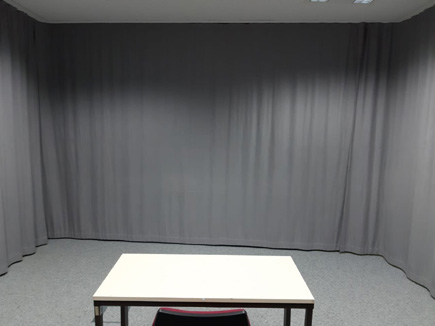
\includegraphics[scale=1]{./images/fig2.jpg}
    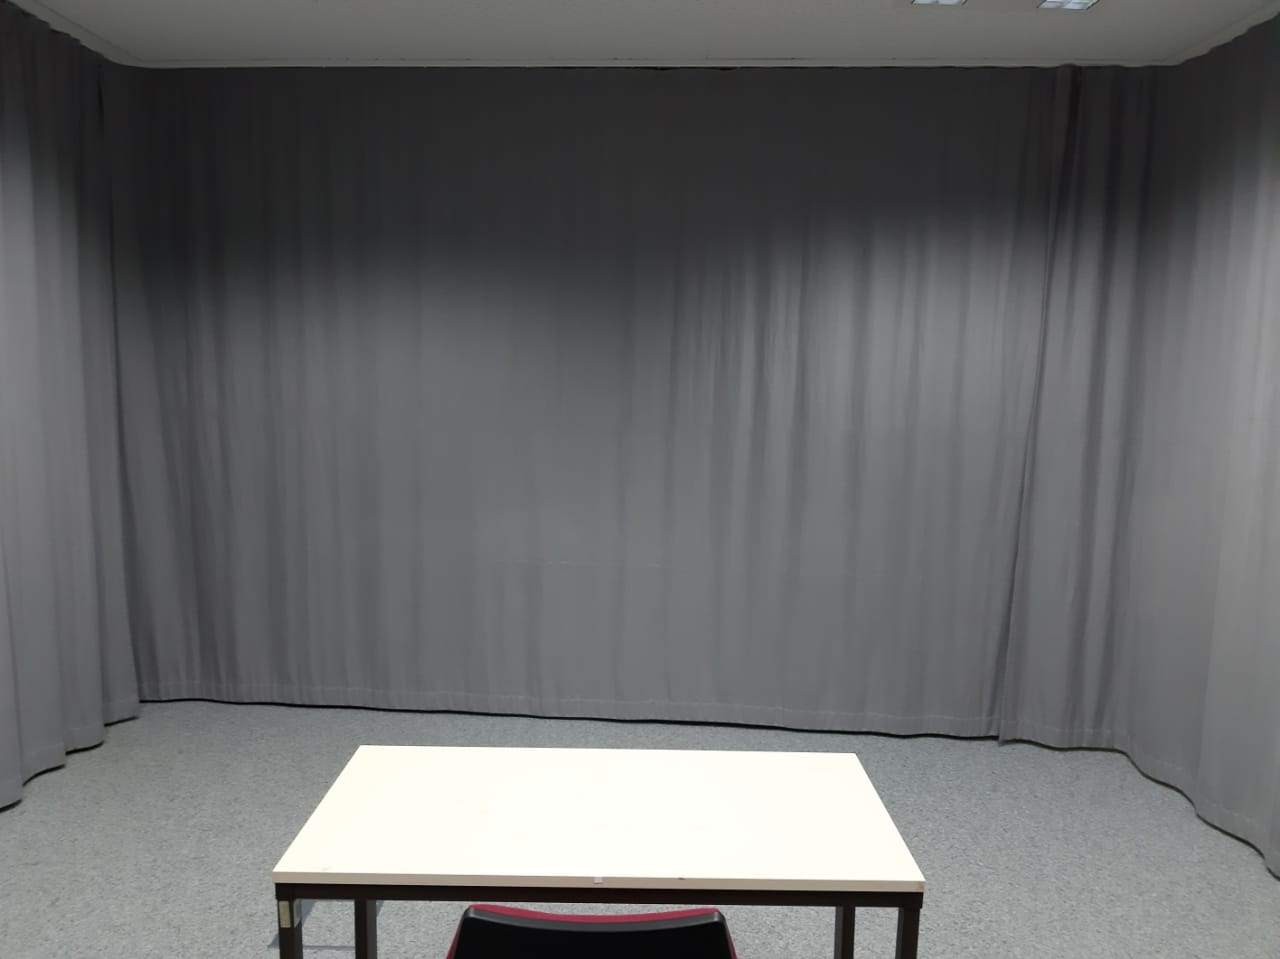
\includegraphics[width=0.8\textwidth]{./images/fig2.jpeg}
    \caption{Audiovisual test lab of the Institute of Media Technology}
    \label{fig:fig2}
\end{figure}

Apart from these elements, the best possible lighting scenario has to be generated to replicate the environment. Firstly the floor of the room has a carpet which we have created in unity using a real picture of the carpet. Secondly, the roof of the real room is built using textured tiles which are also created in unity using real pictures. Thirdly the table was replicated using internal unity tools of 3D objects. Fourthly the chair is replicated using a free unity asset store, packages. Finally, the curtains were replicated. The process of replication of curtain had two possible methods, to create it from scratch in tools like Unity or blender, or use standard free asset and modify it to fit the needs. As designing and rendering is not primary scope of the project so free assets of blender were used. It was then converted to Unity's standard file format and modified inside Unity. It is also worth mentioning here that curtains were not availble as free asset in Unity asset store.   
The most important aspect to make immersive environment is to create the best possible lighting scenario. The roof of the room where tests are conducted contains multiple light sources with no light from the outside. To replicate such lighting, default light sources which included ambient lighting and directional lighting was not right. The multiple lighting in the roof also created an ambient lighting effect which created a complex shadowing effect. To simulate this kind of lighting we used multiple sources of area lighting. It helped to improve the diffused shadow effect which is created due to multiple lights on the roof. For conducting test it was significant to create multiple scenes, every scene depicting a particular test scenario. Following (Figure\ref{fig:replicated}) shows the replicated room in virtual environment\par
\begin{figure}[h]
    \centering
    %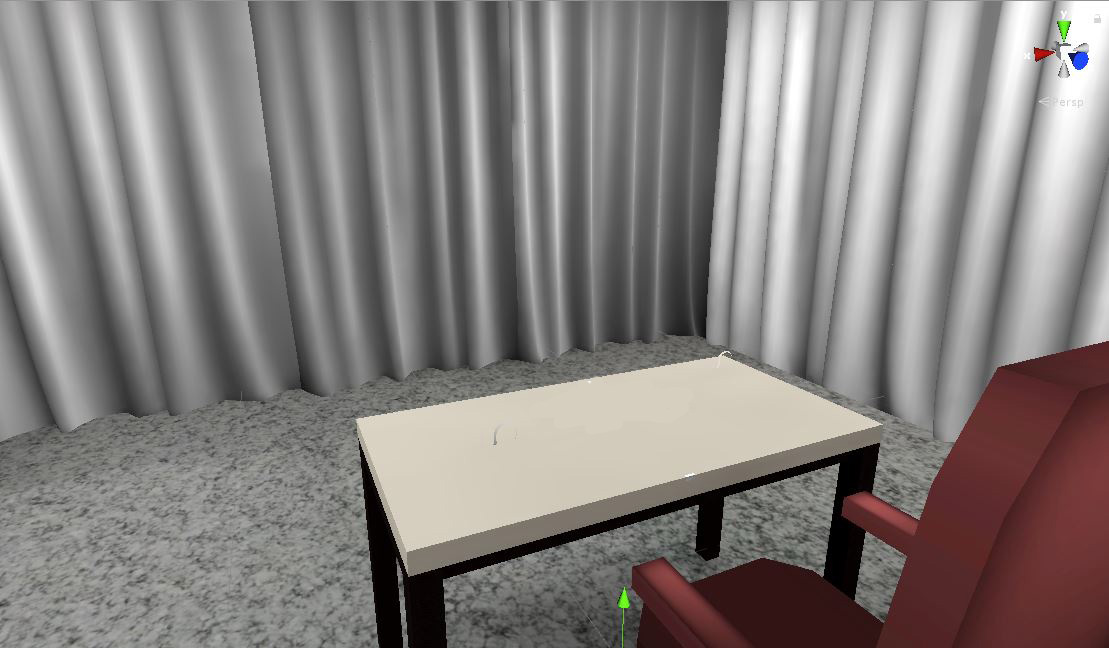
\includegraphics[scale=1]{./images/replicated.jpg}
    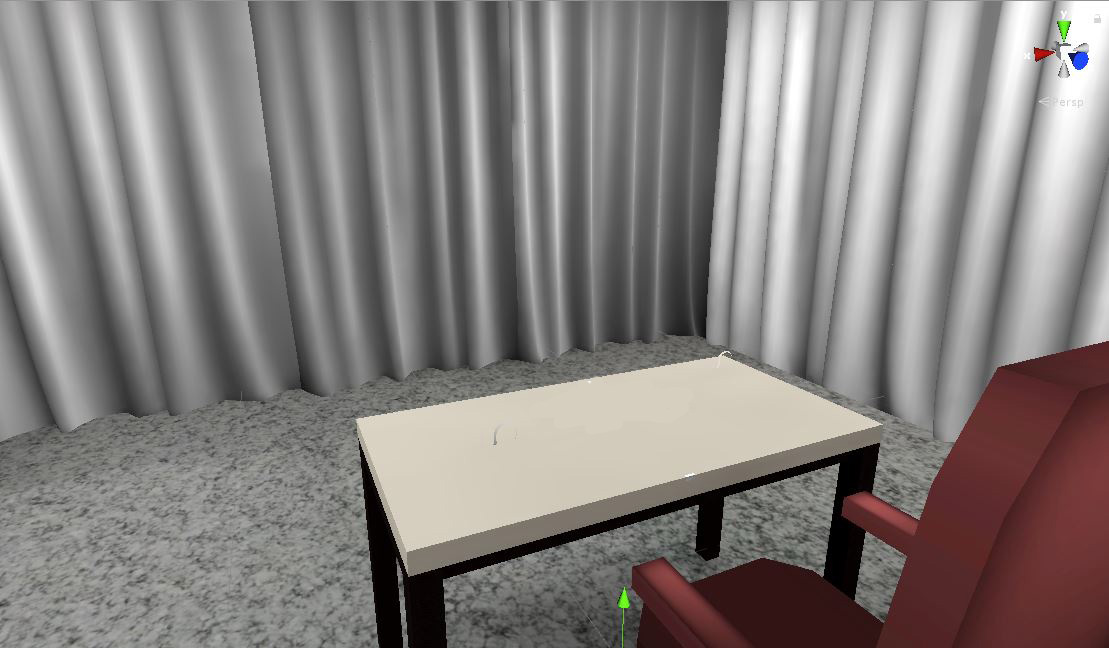
\includegraphics[width=0.8\textwidth]{./images/replicated.jpg}
    \caption{Replicated Room}
    \label{fig:replicated}
\end{figure}
Two controllers and one tracker was used in the tests. First controller was used to manually calibrate the table in virtual environment if it was having offset with respect to real world table. Second controller was attached with the help of velcro to the book which is used in the scenario six, and the tracker was attached to a cylindrical object. It is worth mentioning here that the second controller and the tracker, attached to the book and cylinder respectively, coexisted in the real and virtual environment as shown in (Figure \ref{fig:tracker11}).\par   
\begin{figure}[h]
    \centering
    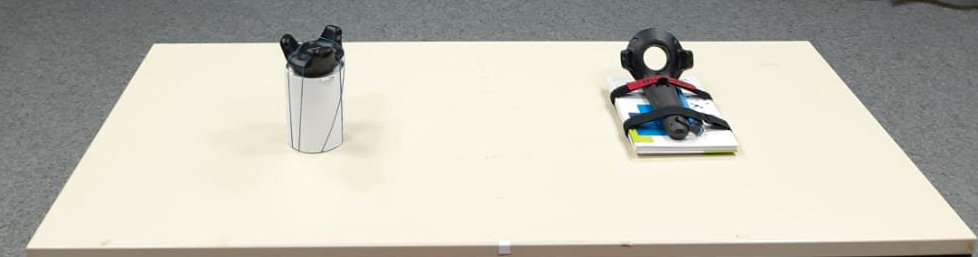
\includegraphics[width=0.8\textwidth]{./images/tracker11.jpg}
    \caption{Second and Third Controller}
    \label{fig:tracker11}
\end{figure}

For our experiment participants were seated in a chair and they were allowed free movement of the head and arm while restricting them to do every task while sitting on a chair. Participants were instructed not to move the position of chair. The height of the chair could be adjusted to make the participant feel comfortable. Participants were allowed to reach the objects on the table with their hands. All the activities required one hand to complete the task.
A table was placed in front of the chair. The size of the table was 120 cm x 60 cm. And the height of the table was 70 cm. Target objects were placed on the table at different distances. 
We used two lighthouses placed 4 m apart. It is observed that if the lighthouse is placed in a way that its shadow is cast on the controller devices then there is more tracking error. The lighthouses are placed in special configuration to have least error while tracking. And the configuration was that the lighthouses were on both sides of the table as shown in the (Figure \ref{fig:lighthouses1}). The height of the lighthouse was 2.5 m and they pointed downward towards the table at an angle of 45$^{\circ}$.
HTC vive Pro HMD was connected to the computer. 

\begin{figure}[h]
    \centering
    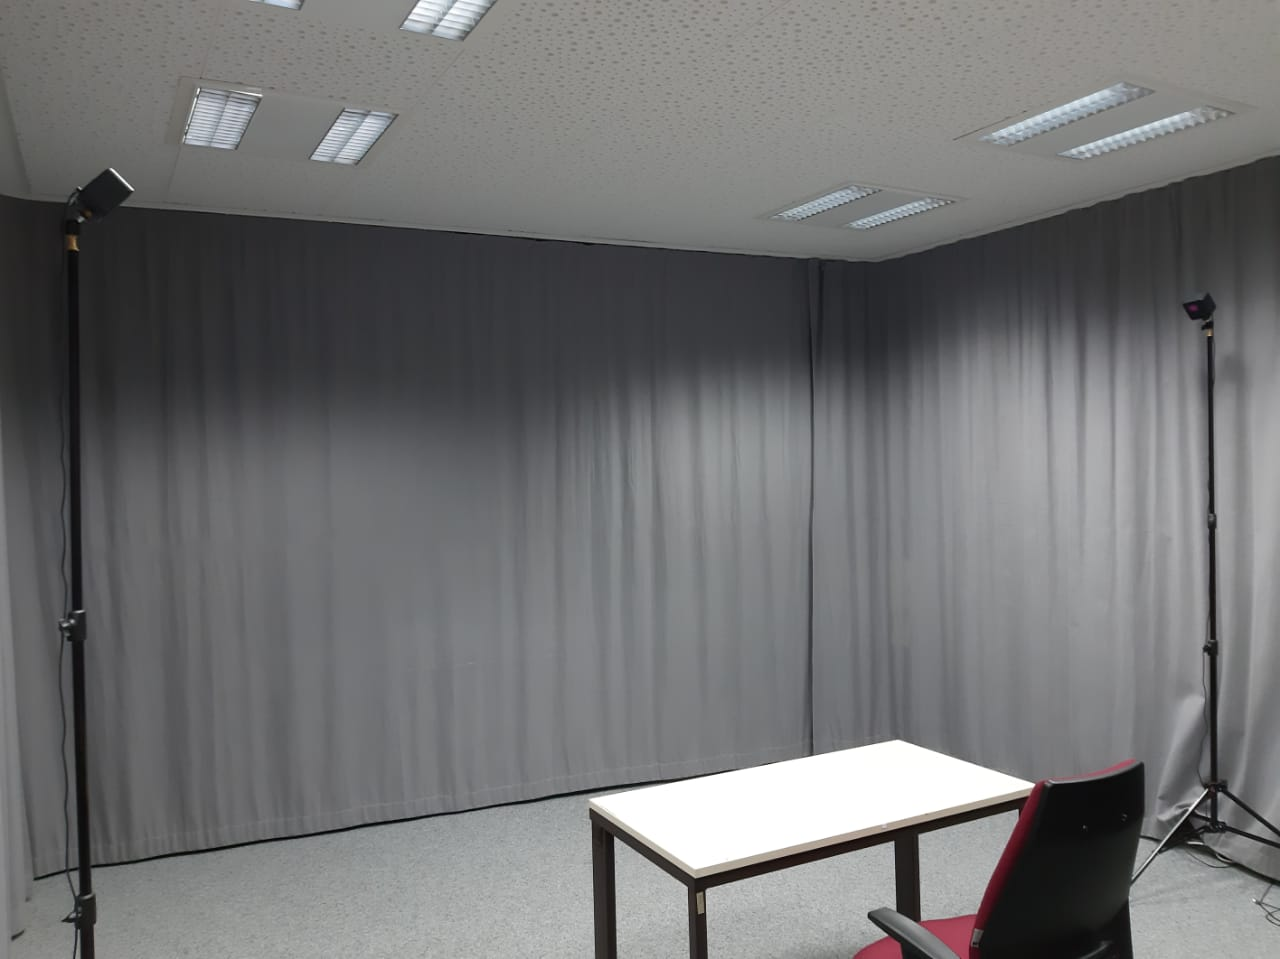
\includegraphics[width=0.8\textwidth]{./images/lighthouses1.jpeg}
    \caption{Lighthouses}
    \label{fig:lighthouses1}
\end{figure}
 



\chapter{Test Design}
\label{sec:Test Design}
The virtual environment (VE) displayed in the HMDs was made to be a rough, non-photorealistic
match of the dimensions, color, and visual texture of the real environment (RE). 19 Participants
were recruited from a university campus, 15 men and 4 women ranging in age from 23 to
33 (Mean=26.31 ,Median=26). On average, the participants were able to complete the subjective test in 45 to 50 mins.
At first, participants were given a test protocol form, they were asked to fill their personal details and question related to their previous experience with HMD. A question regarding their previous experience with HMD was asked i.e., “Do you have previous experiences in using so-called Head-Mounted Displays (HMDs)?”. This question will help to understand the impact of user experience with HMD on the subjective tests. There were four options given to participants for this question. The option started with no experience at all that is I have never watched VR video using an HMD so far. The second option was first experience made i.e. an HMD has been used already one to three times. Third option was extended experience i.e. an HMD has been used at least four times and VR video
content beyond the test series of TU Ilmenau has been seen. And the fourth option was extensive experience an HMD has been used more than ten times and VR video content beyond
the test series of TU Ilmenau has been seen, possibly an own HMD at home. Then the participants were briefed about the study objective, risks of the experiment and privacy.
The were also informed test can be aborted at anytime without reasons. After the initial documentation, six subjective sessions were carried out. The complete questionnaire are attached in the appendix A.
 


\section{Session One: Average Time Calculation Test}
In the first session, an average time is calculated for a given task. The subject was seated on a chair and a table was placed in front of the subject. The position of chair was fixed and the subject was instructed not to move the chair position. The average individual time required to complete the task in the real world was calculated. This time calculation was later used as a baseline to compare it with a similar task performed in the virtual world in the later sessions. 
A task was explained in which the subject had to place the cylinder on the marker. The subject was instructed to place the cylinder in the first attempt. This process was repeated three times and time required to place each object on the marker was noted. An average time of this task was calculated. Setup of the task can be seen as in (Figure \ref{fig:fig3}).
\begin{figure}[h]
    \centering
    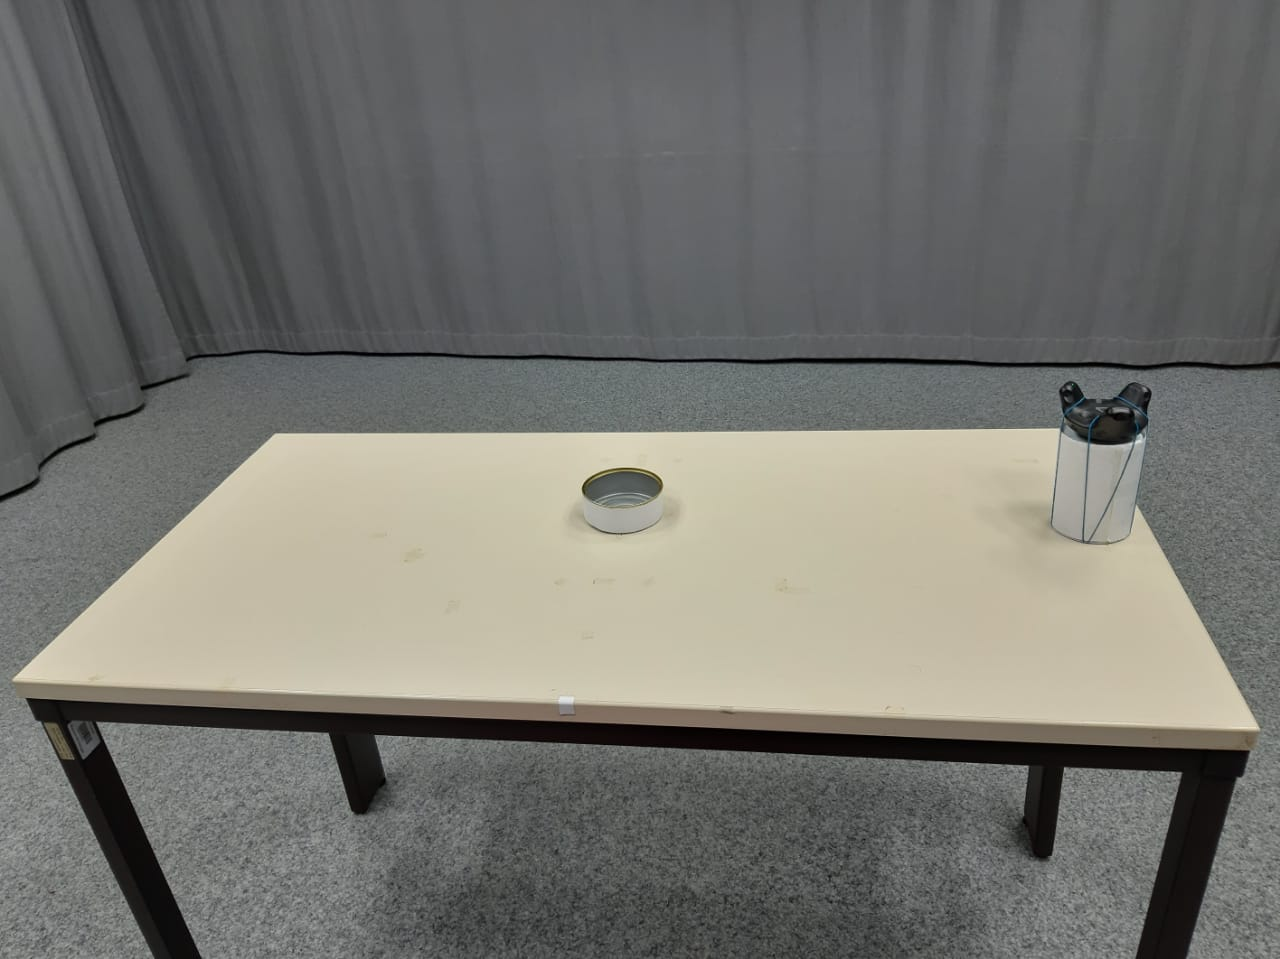
\includegraphics[width=0.8\textwidth]{./images/fig3.jpeg}
    \caption{Session One Setup}
    \label{fig:fig3}
\end{figure}

\section{Session Two: Immersion Test}
In the second session, subject was introduced to the VE by wearing an HMD. The purpose
of this test is to inquire the immersion level of the subject, and comfort level of video viewing in the virtual reality. It also aimed for the subject to adapt to the virtual environment. Before the test began subject was asked to fill a pre-questionnaire of simulator sickness in VR. To have a general view if any symptoms of simulator sickness existed before the test started, three simulator sickness questions were asked. These questions gave an overview of the subjects health. These simulator sickness questions were also asked after every virtual environment test. This helped to observe any impact on the health of participant due to VE test. The simulator sickness questions were, how is the level of dizziness? how is the level of headache? and how is the level of eyestrain?. The purpose of asking these questions was to have a general idea if the subject has symptoms of motion sickness prior to the test in VE. The experimenter made sure that the rating procedure was understood before the experiment began. Then the subjects were given instructions
about what they will view in virtual reality. In the virtual environment a room, which resembled the real room was shown to the subject. The participants stayed in the VE for two minutes. They were instructed to look around in the virtual
environment and judge the level of resemblance and immersion of real and virtual world after the VE session was over. A question was asked, “what was the level of immersion and resemblance of virtual world on a scale from 1 to 5?”. The options were no immersion, slight immersion, moderate, immersive and highly immersive. These options were explained to the user before answering the question. In the virtual environment
subject was shown a video on a flat display. The display was placed on the table in front of the subject in the VE. A two minute video of cartoon big buck bunny with the audio was displayed on the flat display inside the VE. After the session was over, the second question asked was how much comfortable was video viewing in virtual reality on a scale of 1 to 5?. 1 means not at all, 2 means slightly, 3 means moderate, 4 means comfortable and 5 means highly comfortable. Post simulator sickness questions were also asked after the session in the virtual environment.
 
\begin{figure}[h]
    \centering
    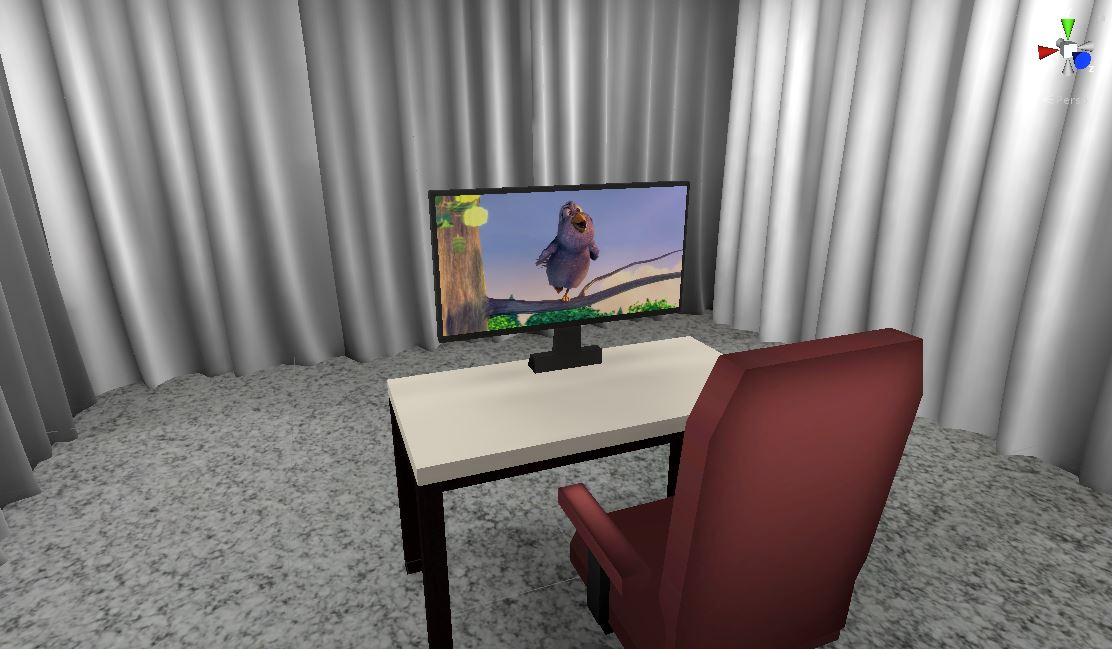
\includegraphics[width=0.8\textwidth]{./images/fig4.jpeg}
    \caption{Virtual Reality Video Experience}
    \label{fig:fig4}
\end{figure}
\section{Session Three: Verbal Distance Estimation Test}
In the third session, the subject had to do distance estimation of objects in real and virtual world. 10 participants estimated the distance first in the real world and then in the virtual world. 8 participants estimated the distance first in the virtual world and then in the real world. The objects for distance estimation were placed on the table in front of the subject. Instructions were given before the start of the test. A physical scale in cm was shown to the subject. The size of scale was 30 cm. The scale was shown, so that, they get an idea of the measurement. The size of the table was also mentioned during the instructions. In this experiment three different objects were used. Each object was placed in two different locations. The three objects were box, cylinder and ball. There was a reference point marked on the table. And the subject had to estimate the distance from that reference point to the face of the object. All of this was explained before the test began. Box was placed in two different locations in vertical direction (i.e. in y-axis direction) on the table. The distances from the referece point to object were chosen randomly, so that the subjects have to judge a new value every time. The first location was 20cm from the reference point and the second location was 40cm from the reference point. Cylinder was placed in two different locations in horizontal direction (i.e. in x-axis direction) on the table. The first location was 30cm on the right from the reference point and the second location was 50cm on the left from the reference point. Ball was placed in two different locations in vertical and horizontal direction (i.e. in x and y axis) on the table. The first location was 50cm in x-axis and 50 cm in y-axis from the reference point and the second location was 30cm in x-axis and 30cm in y-axis from the reference point. The subject estimated the distances verbally and the experimenter noted the distances on a form. Position of objects in real and virtual world were similar but the sequence of objects was randomized. After the distance estimation in VE, subjects were asked SS questions. Following (Figure \ref{fig:fig5}) and (Figure \ref{fig:fig51}) show real and vitual environment respectively. 
\begin{figure}[h]
    \centering
    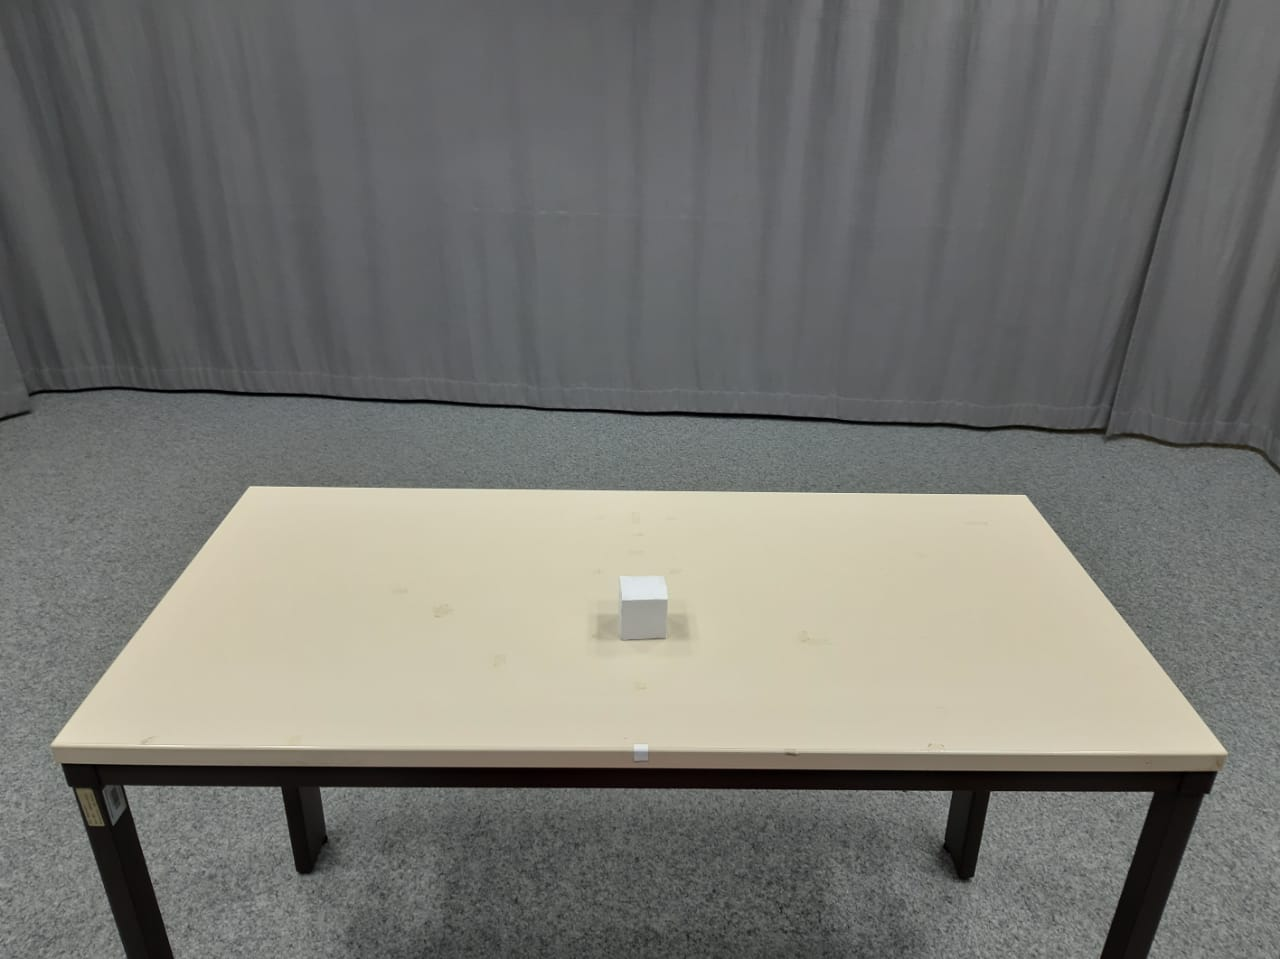
\includegraphics[width=0.8\textwidth]{./images/fig5.jpeg}
    \caption{Real World}
    \label{fig:fig5}
\end{figure}
\begin{figure}[h]
    \centering
    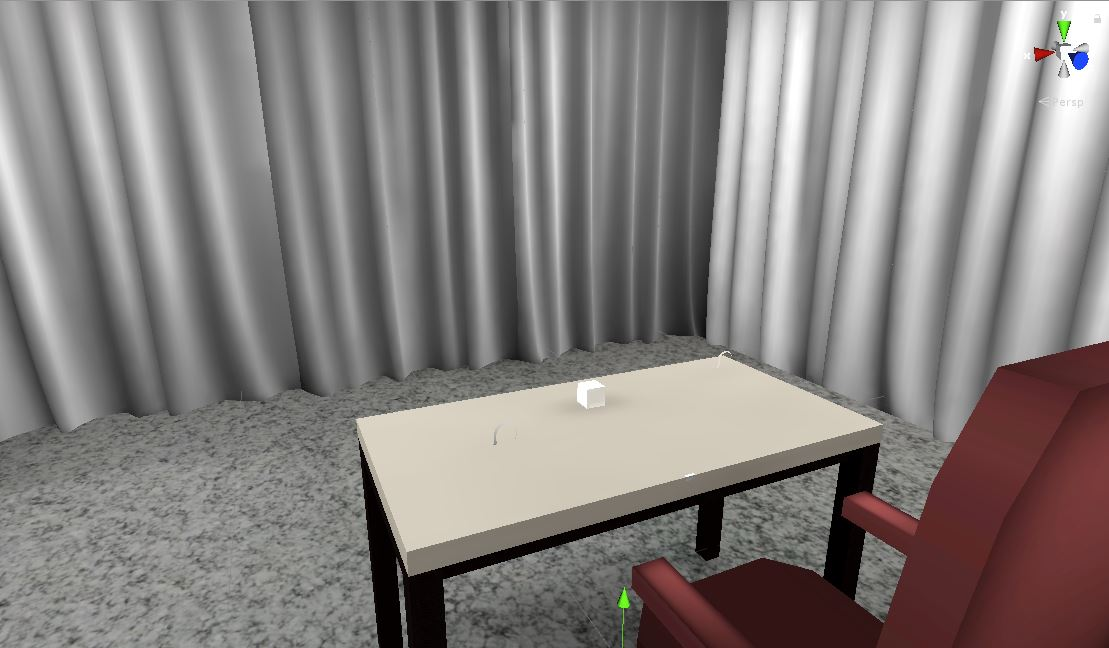
\includegraphics[width=0.8\textwidth]{./images/fig51.jpeg}
    \caption{Virtual World}
    \label{fig:fig51}
\end{figure}
\section{Session Four: Blind Verbal Distance Estimation Test}
The fourth session was blind verbal distance estimation, the subject had to do distance estimation of objects in real and virtual world. Participants had to close their eyes after viewing the object for 5 seconds in the real world. And in the virtual world the screen was blacked out after viewing the object for 5 seconds. After the participants closed their eyes or the screen blacked out in VE, participants had to estimate the distance verbally. 10 participants estimated the distance first in the real world and then in the virtual world. 8 participants estimated the distance first in the virtual world and then in the real world. The objects for distance estimation were placed on the table in front of the subject. Instructions were given before the start of the test. A physical scale in cm was shown to the subject. The size of scale was 30 cm. The scale was shown, so that, they get an idea of the measurement. The size of the table was also mentioned during the instructions. In this experiment three different objects were used. Each object was placed in two different locations. The three objects were
box, cylinder and ball. There was a reference point marked on the table. And the subject had to estimate the distance from that reference point to the face of the object. All of this was explained before the test began. Box was placed in two different locations in vertical direction (i.e. in y-axis direction) on the table. The first location was 10cm from the reference point and the second location was 50cm from the reference point. Cylinder was placed in two different locations in horizontal direction (i.e. in x-axis direction) on the table. The first location was 15cm on the right from the reference point and the second location was 35cm on the left from the reference point. Ball was placed in two different locations in vertical and horizontal
direction (i.e. in x and y axis) on the table. The first location was 40cm in x-axis and 40 cm in y-axis from the reference point and the second location was 15cm in x-axis and 15cm in y-axis from the reference point. The subject estimated the distances verbally and the experimenter noted the distances on a form. Position of objects in real and virtual world were similar but the sequence of objects was randomized. After the distance estimation in VE, subjects were asked SS questions. 


%\begin{figure}[h]
%    \centering
%    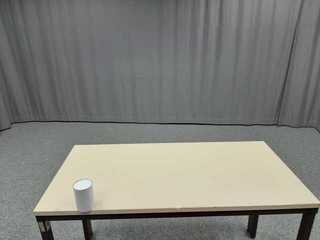
\includegraphics[scale=1]{./images/fig6.jpeg}
%    \caption{Seesion Four}
%    \label{fig:ex1}
%\end{figure}

\section{Session Five: Nested Object Placement Test}
The fifth session was nested object placement, this experiment was focused on finding perceivable distance difference in near field. Or at what point the distance difference is noticeable to the subject in the near field. The instructions were given to place object A which was a cylinder inside object B which was a ring. Following (Figure \ref{fig:fig7}) shows the setup in virtual environment. 
\begin{figure}[h]
    \centering
    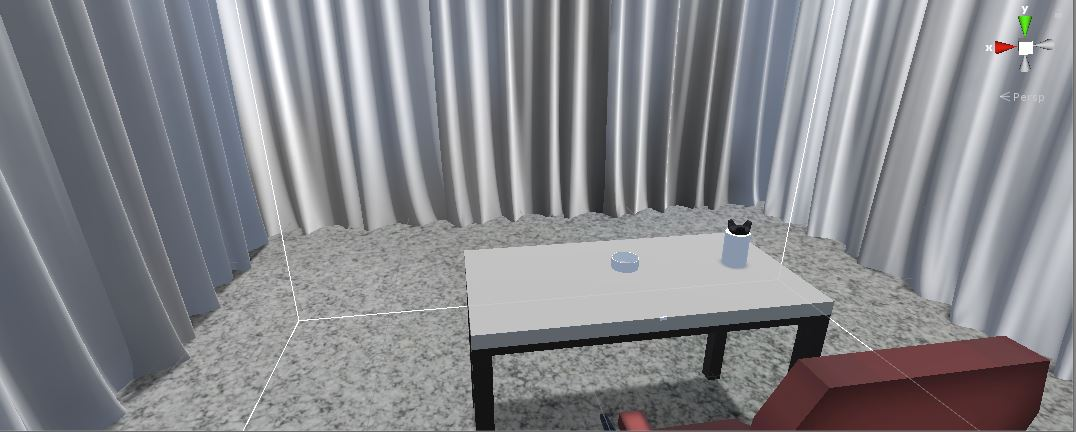
\includegraphics[width=0.8\textwidth]{./images/fig7.jpeg}
    \caption{Session Five}
    \label{fig:fig7}
\end{figure}
A question was asked after performing the task, i.e. what is the degree of confusion while performing the task on a scale from 1 to 5. 1 means no confusion, 2 means
slightly confused, 3 means confused, 4 means highly confused and 5 means extremely confused. This task was repeated five times. Each time the ring (object B) was shifted to 1 cm from the original location in the virtual world. But its physical location in the real world remained the same. The shift position of the object was randomized. The first shift was on the right of the original position of ring. Second shift was on the left of the original position. Third shift was again on the right of the original position and finally the fourth shift was in the downward direction i.e. towards the participant. The average time to perform the task in the real world was calculated in the session 1 and used for comparing with the time required to complete the task in the virtual world. After the virtual environment experiment there was a SS questionnaire. 

\section{Session Six: Play Area Test}
The last session was a play area in the virtual world. The subject had to interact with the two objects, first object was a book and second object was a cylinder. There were two markers one for the book and other for the cylinder on the table both in real and VE. Participants had to pick and place the objects on the markers. Trackers were attached with the objects, so that, real time tracking of the objects is visible in the virtual world as can be seen in (Figure \ref{fig:fig81}) and (Figure \ref{fig:fig8}). The experiment was first done in the real world and individual time was noted for placing each object on the marker. Then the experiment was repeated in the VE. In VE the participant was able to see the markers and objects on the table. Participant was instructed to pick the objects and place it on the markers. Also, leave the object after placing it on the marker. Time was also noted in VE for placing the object on markers. After the participant placed the object in VE, experimenter noted the offset of the object between the virtual and real environment. 

\begin{figure}[h]
    \centering
    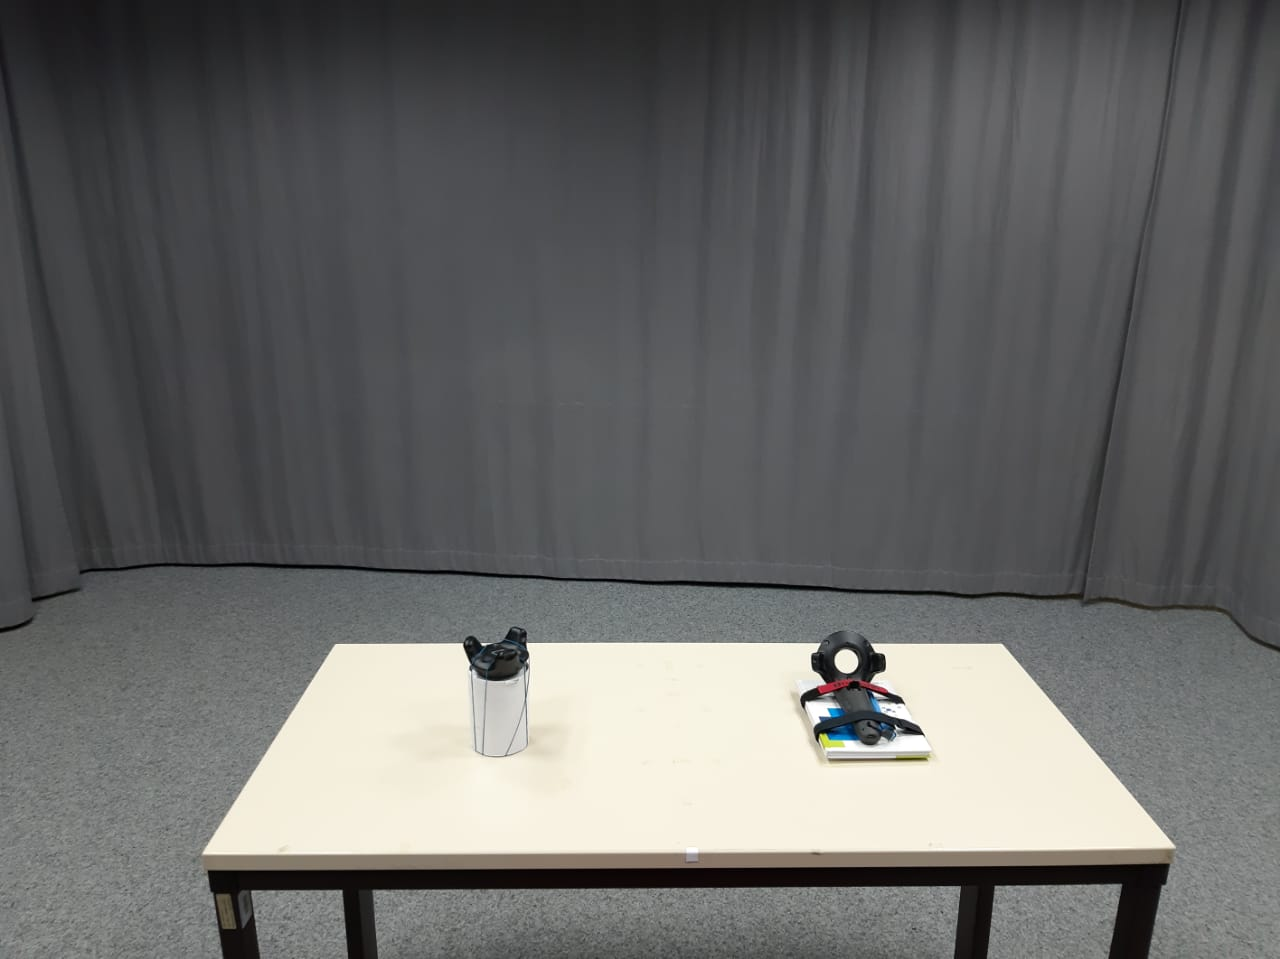
\includegraphics[width=0.8\textwidth]{./images/fig81.jpeg}
    \caption{Real World}
    \label{fig:fig81}
\end{figure}
\begin{figure}[h]
    \centering
    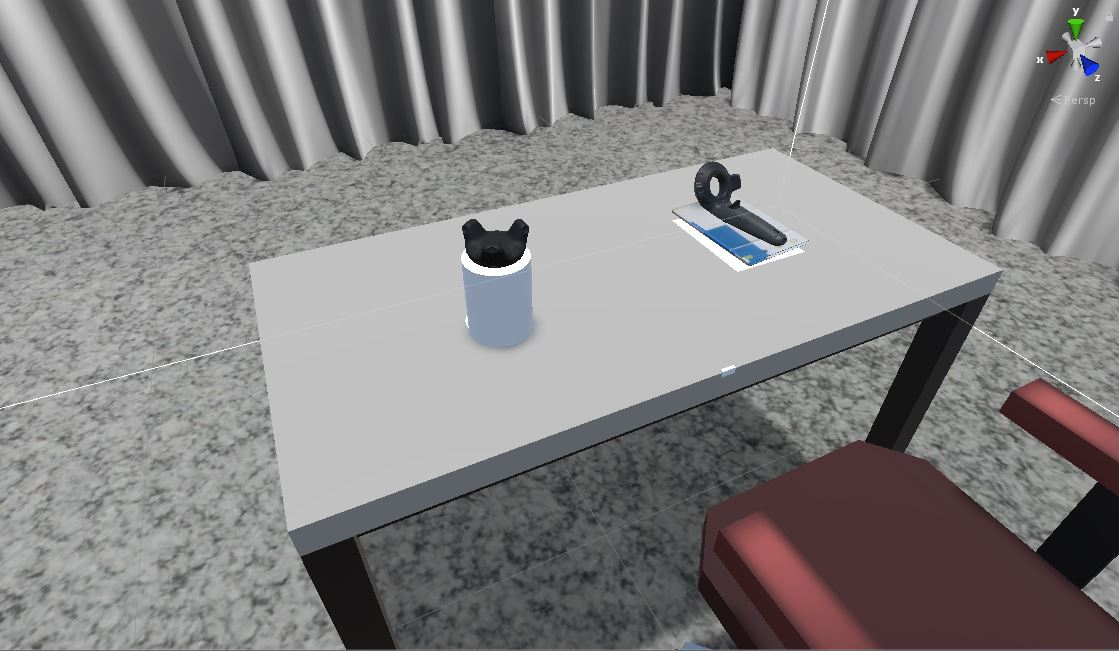
\includegraphics[width=0.8\textwidth]{./images/fig8.jpeg}
    \caption{Virtual World}
    \label{fig:fig8}
\end{figure}

\chapter{Evaluation}
\label{sec:Evaluation}
In this chapter, the results are shown by the order of sessions conducted with the participants. The results are evaluated using statistical methods of mean, t-test and ANOVA, it is then followed by tables and graph representation. 
\section{Pre Screening}
The evaluation of pre screening questionnaire about previous experience with HMD showed two people had extensive experience, four had extended experience, one had made first experience before and 13 had no previous experience. Visual test was also included in the protocol. Snellen chart was used to measure the visual acuity. 18 out of 19 participants passed the visual test. The average time taken to complete the task in session 1 was 5.3s. While performing the same task in VE participants on average took 6.72s.

\section{Immersion and Video Viewing}
Out of 18 participants 4 participants felt highly immersive, 12 participants felt immersive and 2 participants felt moderately immersive in virtual environment.
For analyzing the results mean opinion scores (MOS) and associated 95\% confidence intervals have been calculated for the questions and test conditions. The figure below shows the MOS of previous experience with HMD, resemblance of physical and virtual world and degree of comfort while viewing video in VE. Out of 18 participants, 9 were highly comfortable, 8 were comfortable and 1 was moderately comfortable.\par 
\begin{figure}[h]
    \centering
    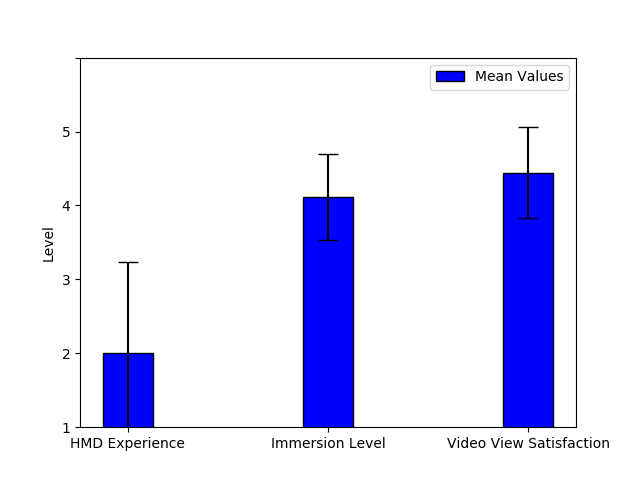
\includegraphics[width=0.8\textwidth]{./images/immersion1.png}
    \caption{Mean HMD Experience, Immersion and Video Satisfaction with 95\% confidence interval}
    \label{fig:immersion1}
\end{figure}
\section{Verbal Distance Estimation}
In verbal distance estimation 18 participants in total made 108 estimations in real world and 108 estimation in virtual world. The results of real world distance estimation were following, for box location at 20cm, 7 out of 18 people underestimated the distance, 5 subjects overestimated and 6 subjects judged the distance correctly. When the box was located at 40cm, 5 out of 18 people underestimated the distance, 6 subjects overestimated and 7 subjects judged the distance correctly. Whereas when the cylinder was located at 30cm, 9 out of 18 people underestimated the distance, 6 subjects overestimated and 3 subjects judged the distance correctly. Cylinder with the distance of 50cm, 8 out of 18 people underestimated the distance, 4 subjects overestimated and 6 subjects judged the distance correctly. While the ball at distance of (50,50) cm, 16 out of 18 people overestimated the distance and 2 subjects judged the distance correctly. For ball location at (30,30) cm, 17 out of 18 people overestimated the distance and 1 subject judged the distance correctly. The results of distance estimation in the virtual world are following, while the box was located at 20cm, 6 out of 18 people underestimated the distance, 6 subjects overestimated and 6 subjects judged the distance correctly. Whereas at 40cm, 4 out of 18 people underestimated the distance, 8 subjects overestimated and 6 subjects judged the distance correctly. The cylinder located at 30cm, 7 out of 18 people underestimated the distance, 7 subjects overestimated and 4 subjects judged the distance correctly. Whereas at 50cm, 10 out of 18 people underestimated the distance, 3 subjects overestimated and 5 subjects judged the distance correctly. The ball located at distance of (50,50) cm, 0 out of 18 people underestimated the distance, 15 subjects overestimated and 3 subjects judged the distance correctly. For ball location at (30,30) cm, 1 out of 18 people underestimated the distance, 16 subjects overestimated and 1 subject judged the distance correctly.

As shown in Table \ref{tab:Real World Estimates1}, in the real world, on average 51\% underestimations,
27\% overestimation and 22\% hits were registered. As shown in Table \ref{tab:Virtual World Estimates1}, In the virtual environment, on average 51\% underestimation, 28.7\% overestimation and 20.3\% hits were registered overall conditions. To test the hypothesis that real and virtual environment shows statistically no significant different means in verbal distance estimation, a paired t-test was performed, the two-tail p-value for this test was p= 0.97146 and t= -0.03584. Since the p-value is greater than 0.05, it can be concluded that there is no statistically significant difference between the means of real and virtual world distance estimation.\par

\begin{table}
    \centering
    \begin{tabular}{|3|1|1|1|1|}
        \toprule
        Object Type & Distances & Underestimation & Overestimation & Hit \\
        \midrule
        Box & 20 cm &
                7 & 5 & 6 \\
                \hline
        Box & 40 cm &
                5 & 6 & 7 \\
                \hline
        Cylinder & 30 cm &
                9 & 6 & 3 \\
                \hline
        Cylinder & 50 cm &
                8 & 4 & 6 \\
                \hline
        Ball & 70 cm &
        		12 & 4 & 2 \\
        		\hline
        ball & 42 cm &
        		14 & 4 & 0 \\
        \midrule		
        Total & 
        		& 55 & 29 & 24 \\				        
        \bottomrule
    \end{tabular}
    \caption{Real World Estimates}
    \label{tab:Real World Estimates1}
\end{table}

\begin{table}
    \centering
    \begin{tabular}{|3|1|1|1|1|}
        \toprule
        Object Type & Distances & Underestimation & Overestimation & Hit \\
        \midrule
        Box & 20 cm &
                6 & 6 & 6 \\
                \hline
        Box & 40 cm &
                4 & 8 & 6 \\
                \hline
        Cylinder & 30 cm &
                7 & 7 & 4 \\
                \hline
        Cylinder & 50 cm &
                10 & 3 & 5 \\
                \hline
        Ball & 70 cm &
        		14 & 3 & 1 \\
        		\hline
        ball & 42 cm &
        		14 & 4 & 0 \\
        \midrule		
        Total & 
        		& 55 & 31 & 22 \\				        
        \bottomrule
    \end{tabular}
    \caption{Virtual World Estimates}
    \label{tab:Virtual World Estimates1}
\end{table}
 
The three objects used in estimations are differently displaced on the table. The box is linearly displaced along the y-axis direction from the reference point, the cylinder is displaced along the x-axis direction and ball is displaced along x and y axis (i.e diagonally from the reference point). To test the hypothesis that there was statistically no significant difference when estimating the distance in a particular direction ANOVA was performed. ANOVA results revealed significant impact of object location on distance estimation, F(2,105)= 3.9286, p=0.022 in real world and F(2,105) = 5.771, p = 0.004 in virtual world. It can also be seen in the Figure \ref{fig:graph1} that for both real and virtual environment object direction from the reference point increases the error in judgment.  
\begin{figure}[h]
    \centering
    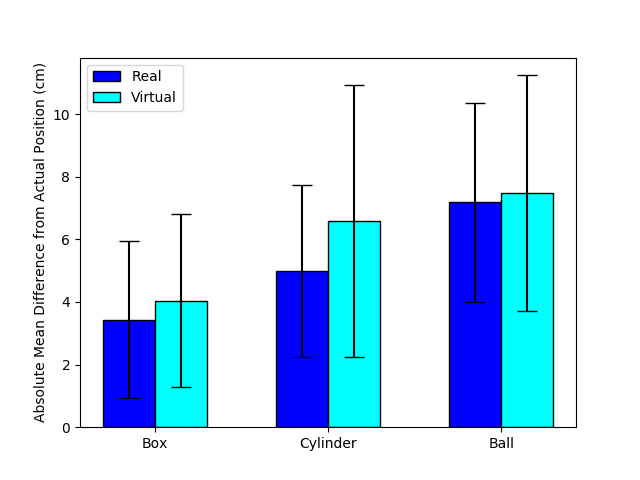
\includegraphics[width=0.8\textwidth]{./images/verbal101.png}
    \caption{Real Versus Virtual Mean with 95\% Confidence Interval}
    \label{fig:graph1}
\end{figure}
\section{Blind Distance Estimation}  
In blind verbal distance estimation 18 participants in total made 108 estimations in real world and 108 estimation in virtual world. The results of real world distance estimation were following, for box location at 10cm, 6 out of 18 people underestimated the distance, 4 subjects overestimated and 8 subjects judged the distance correctly. Whereas at 50cm distance, 2 out of 18 people underestimated the distance, 11 subjects overestimated and 5 subjects judged the distance correctly. The cylinder located at 15cm, 7 out of 18 people underestimated the distance, 7 subjects overestimated and 4 subjects judged the distance correctly. Whereas at 35cm, 6 out of 18 people underestimated the distance, 9 subjects overestimated and 3 subjects judged the distance correctly. The ball located at (40,40) cm distance, 1 out of 18 people underestimated the distance, 15 overestimated the distance and 2 subjects judged the distance correctly. Whereas at location (15,15) cm, 2 out of 18 people overestimated the distance, 12 overestimated the distance and 4 subjects judged the distance correctly. 
The results of distance estimation in the virtual world are following, for box location at 10cm, 8 out of 18 people underestimated the distance, 3 subjects overestimated and 7 subjects judged the distance correctly. At 50cm, 3 out of 18 people underestimated the distance, 9 subjects overestimated and 6 subjects judged the distance correctly. The cylinder located at 15cm, 7 out of 18 people underestimated the distance, 6 subjects overestimated and 5 subjects judged the distance correctly. Whereas at 35cm, 15 out of 18 people underestimated the distance and 3 subjects overestimated. For ball location at (40,40) cm, 2 out of 18 people underestimated the distance, 15 subjects overestimated and 1 subjects judged
the distance correctly. For the ball location at (15,15) cm, 1 out of 18 people underestimated the distance, 12 subjects overestimated and 5 subjects judged the distance correctly. As shown in Table \ref{tab:Real World Estimates2}, in the real world, on average 41.5\% underestimations, 39\% overestimation and 19.5\% hits were registered. As shown in Table \ref{tab:Virtual World Estimates2}, In the virtual environment, on average 55.5\% underestimation, 28\% overestimation and 16.5\% hits were registered overall conditions. To test the hypothesis that real and virtual environment shows statistically significant different means in blind distance estimation, a paired t-test was performed, the two-tail p-value for this test was p= 0.0146 and t= 2.4823. Since the p-value is 0.0146, i.e. less than 0.05, it can be concluded that there is a significant difference when estimating the distance in real and virtual environment. 
\begin{table}
    \centering
    \begin{tabular}{|3|1|1|1|1|}
        \toprule
        Object Type & Distances & Underestimation & Overestimation & Hit \\
        \midrule
        Box & 10 cm &
                6 & 4 & 8 \\
                \hline
        Box & 50 cm &
                2 & 11 & 5 \\
                \hline
        Cylinder & 15 cm &
                7 & 7 & 4 \\
                \hline
        Cylinder & 35 cm &
                6 & 9 & 3 \\
                \hline
        Ball & 56 cm &
        		10 & 8 & 0 \\
        		\hline
        ball & 21 cm &
        		14 & 3 & 1 \\
        \midrule		
        Total & 
        		&45 & 42 & 21 \\				        
        \bottomrule
    \end{tabular}
    \caption{Real World Estimates}
    \label{tab:Real World Estimates2}
\end{table}

\begin{table}
    \centering
    \begin{tabular}{|3|1|1|1|1|}
        \toprule
        Object Type & Distances & Underestimation & Overestimation & Hit \\
        \midrule
        Box & 10 cm &
                8 & 3 & 7 \\
                \hline
        Box & 50 cm &
                3 & 9 & 6 \\
                \hline
        Cylinder & 15 cm &
                7 & 6 & 5 \\
                \hline
        Cylinder & 35 cm &
                15 & 3 & 0 \\
                \hline
        Ball & 56 cm &
        		12 & 6 & 0 \\
        		\hline
        ball & 21 cm &
        		15 & 3 & 0 \\
        \midrule		
        Total & 
        		&60 & 30 & 18 \\				        
        \bottomrule
    \end{tabular}
    \caption{Virtual World Estimates}
    \label{tab:Virtual World Estimates2}
\end{table}

Objects used for distance estimation in blind tests are differently displaced on the table. To test the hypothesis that there was statistically no significant difference when estimating the distance in a particular direction ANOVA was performed. ANOVA results revealed significant impact of object location on distance estimation, F(2,105)= 6.042, p=0.0032 in real world and F(2,105) = 5.214, p = 0.0069 in virtual world. As deduced in Figure \ref{fig:graph1}, Figure \ref{fig:graph2} also show the same trend of strong differences of judgement across differend directions.  
\begin{figure}[h]
    \centering
    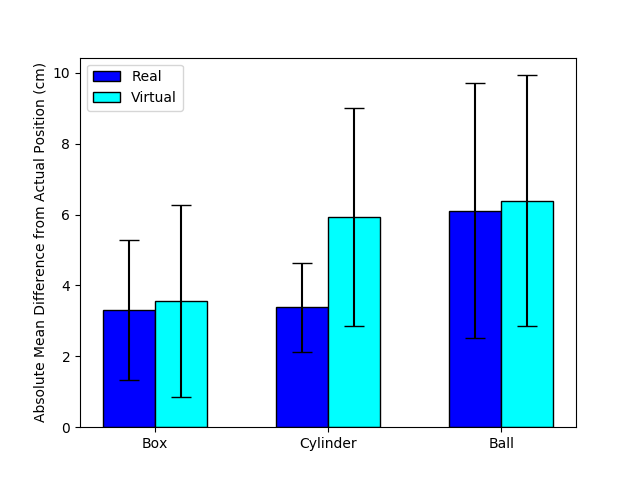
\includegraphics[width=0.8\textwidth]{./images/blind111.png}
    \caption{Real vs Virtual Mean with 95\% Confidence Interval}
    \label{fig:graph2}
\end{figure} 

\section{Nested Object Placement}
Nested object placement test evaluates the distance differences the user experienced while performing the task in the virtual world. The table below shows the grade of confusion (1-5). Participants had against the distance differences in VE. The objects were randomly shifted in the VE. The average time to perform the task in the real world environment was 5.29 seconds. Time
to perform the task in VE was compared with individual’s baseline time calculated in real environment. At orignal position, there was no distance difference in ring (object B) in real and virtual world. 11 out of 18 participants had no confusion in performing the task, 5 participants had slight confusion and 2 participants were confused. When there was 1 cm shift of object B in virtual world, 8 out of 18 participants had no confusion, 7 participants had slight confusion, 1 participant was confused and 2 participants were highly confused. While 2 cm shift of object B in virtual world, 1 out of 18 participants had no confusion, 5 participants had slight confusion, 7 participants were confused, 4 participants were highly confused and 1 participant was extremely confused. Whereas at 3 cm shift of object B in virtual world, 4 out of 18 participants had slight confusion, 8 participants were confused, 3 participants were highly confused and 3 participants were extremely confused. At 4 cm shift, 1 out of 18 participants had no confusion, 4 participants had slight confusion, 6 participants were confused, 4 participants were highly confused and 3 participants were extremely confused.
\begin{table}
    \centering
    \begin{tabular}{|3|1|1|1|}
        \toprule
                   & Mean Confusion & Std of Confusion & Avg Time Difference w.r.t Base line \\
        \midrule
        Orignal &
                1.5 & 0.707 & 1.43 \\
                \hline
        1 cm Displacement &
                1.833 & 0.985 & 2.13 \\
                \hline
        2 cm Displacement &
                2.944 & 0.998 & 5.19 \\
                \hline
        3 cm Displacement &
                3.277 & 1.017 & 4.95 \\
                \hline
        4 cm Displacement &
        		3.22 & 1.165 & 4.30 \\
        			        
        \bottomrule
    \end{tabular}
    \caption{Virtual Environment Object Placement}
    \label{tab:Virtual Environment Object Placement}
\end{table}
\begin{figure}[h]
    \centering
    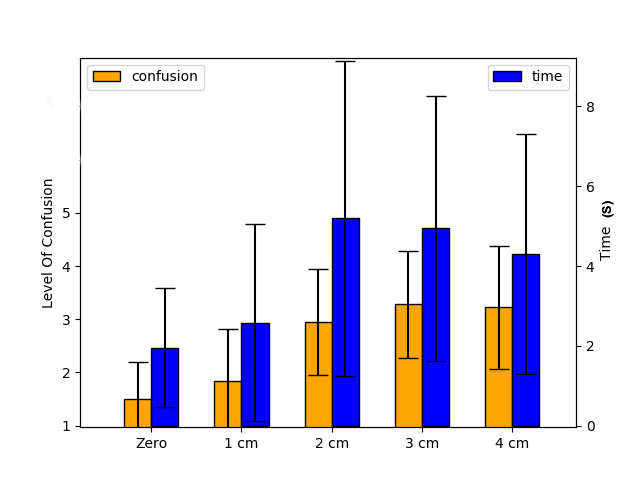
\includegraphics[width=0.8\textwidth]{./images/main_confusion.jpg}
    \caption{Mean Confusion and Mean Time}
    \label{fig:mean confusion}
\end{figure}
The result of session five in terms of mean for the original location i.e. 0cm shift reveal that while performing the task participants felt none to slight confusion. The reason for some participants to feel slight confusion is because of system inaccuracy. The inaccuracies in the system, probably originated from tracking, positional shifts and human errors. The mean values in the Table \ref{tab:Virtual Environment Object Placement} show that confusion increased for participants as the displacement increased. The same pattern is true for the average time difference with respect to baseline time until 2 cm displacement. But after 2
cm there is a slight drop in the average time. The time to perform the task improved on
average from 2 cm to 4 cm, the reason for this improvement lies in the fact that participants learned cognitively that system has a forced inaccuracy. It is worth noting here that mean confusion is highest for participants at 2 cm displacement and after that there is slight drop. The reason for this drop is the same as it is for time, and that is the learning. Motivated by some concern about possible differences in virtual environment confusion between experienced and non experienced users, we then examined our results separately for the two groups. However, we did not find any significant differences in the results. The pearson correlation value between participants confusion and time required to complete the task is R = 0.95. We can see that the two values are positively correlated. This represents a high level of correlation (Figure \ref{fig:corelation}).

\begin{figure}[h]
    \centering
    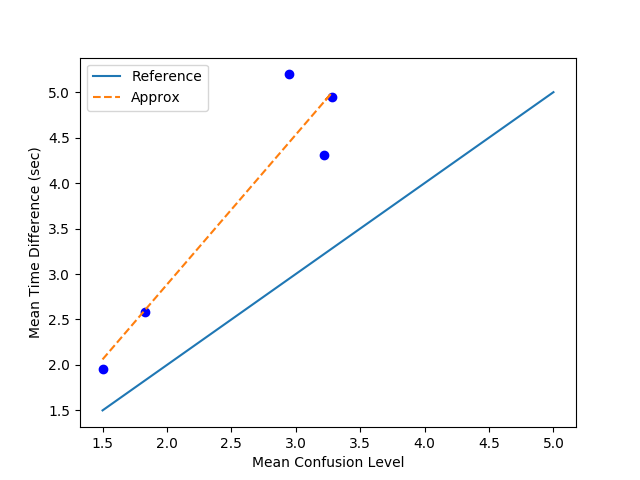
\includegraphics[width=0.8\textwidth]{./images/corelation.png}
    \caption{Coorelation Between Time and Confusion}
    \label{fig:corelation}
\end{figure}

\section{Play Area}
In session six, overall participants placed the objects within +/- 1.5 cm offset from the origin. On average participants took 1.21 seconds more to perform the task in VE. The highest offset while performing the task is 1.5 cm but for most of the participants it was zero. The most probable reason for this shift for small number of participants is the combined positional, tracking and human error. 9 out of 18 participants had no offset and 9 participants had less than +/- 2cm offset. After the experiment in VE SS questionnaire was asked. 

\section{Simulator Sickness}
Before the test began pre simulator sickness questions were asked out of 18 participants 3 participants had slight simulator sickness symptoms. After the first virtual environment session, out of 15 participants that previously had no symptoms of simulator sickness 3 participants felt slight simulator sickness after viewing the video in VR. In verbal distance estimation there was a slight increase in simulator sickness of 2 subjects after the virtual environment test. In blind verbal distance estimation there was a slight increase in simulator sickness of 3 subjects after the virtual environment test. And 5 participants simulator sickness decreased. In session 5, 1 participant felt slight simulator sickness from this experiment and 4 participants that previously had slight discomfort their condition improved. After the final virtual environment test in session 6, the result showed, 13 participants experienced no discomfort and 5 participants experienced slight discomfort. 
\begin{figure}[h]
    \centering
    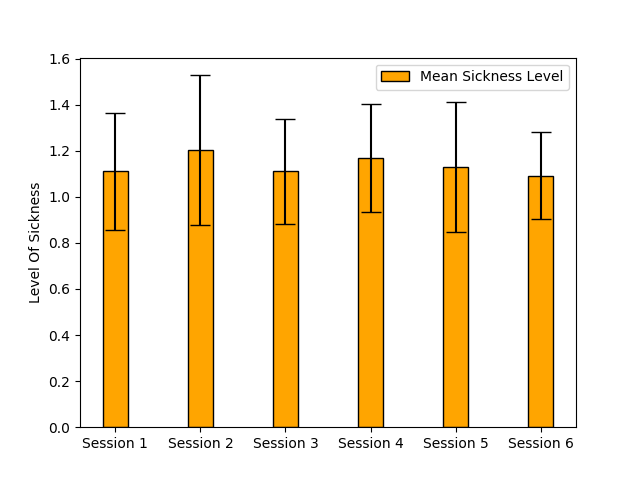
\includegraphics[width=0.8\textwidth]{./images/sickness.png}
    \caption{Simulator Sickness}
    \label{fig:sickness}
\end{figure}
On the basis of these results, we conclude that the virtual experience did not cause severe physical problems and that the objective data are not confounded by discomfort. In the Figure \ref{fig:sickness} the sickness is the measure of headache, dizziness and eyestrain mean values.    

\chapter{Conclusion and Future Work}
\label{sec:Conclusion and Future Work}
The present study is conducted to provide insight in the noticeable distance differences that exists in the near field immersive virtual environment. We tried to answer, what is the distance difference in IVE of a shift between a physical object and the respective object displayed in the virtual environment. Evaluating the results of test systems for investigating the distance differences in IVE for near-field interaction indicates that there is a difference in performance between the real world and the virtual environment. To improve the immersion level of participants, the virtual environment was replicated close to the participant’s real surroundings. Subjective ratings showed that the participants felt highly immersive in the virtual environment.\par 

Overall, virtual and real distances judgment results were similar in the verbal distance estimation test scenario. There was no significant estimation difference between both environments. However, virtual distances were basically underestimated in blind distance estimation and the location of the object in the near field also impacted the distance judgments in both environments. \par 
  
In the evaluation of the distance difference test scenario, a significant confusion was observed when the virtual world was shifted 2cm or more from the real world. Also, the time required to complete the task increased significantly as seen in Figure \ref{fig:mean confusion}. However,  when the shift is increased to 3cm and 4cm the confusion slightly drops and the average time for task completion also improves. The reason for this improvement could lie in the fact that participants learned cognitively that the system has a forced inaccuracy. In addition, when the participants had to pick and place the objects seen in the virtual environment while physically interacting with them in the real world. Overall participants placed the objects within +/- 1.5 cm offset from the origin in the real world. We can conclude from our results that the distance difference of 2cm or more of an object in the real environment and the respective object displayed in the IVE is noticeable by the user. It is important to mention here that these readings are dependent on our system which includes HTC Vive Pro, SteamVR and Unity 3D. \par

Finally, subjective ratings on physical discomfort and general experience in virtual environments were satisfactory. Some participants reported little discomfort. \par

There are many parameters in this study which can be altered or refined to produce different results. There are also chances to enhance the scope of this study. They are briefly covered in the following paragraph\par
There is significant room for improvement in implementation and test design. In the implementation phase we have used two lighthouses and can not add more because it has version 1.0,  with lighthouse version 2.0 more than two can be used which could improve tracking and system error.  It is also possible to go for completely different tracking system e.g. qualisys, optitrack or Advanced Real Time tracking system. Another problem we faced was that for some scenarios in our test condition, tracking of the object was required, which means we wanted dynamic shadowing effect in Unity 3D but the feature is not available for area lighting. Due to this reason, we had to add some directional source of lighting as well, which slightly deteriorated the performance. Better lighting and shadowing can improve IVE which can have an impact on depth perception of participants.  
In the test design, the approach used to minimise the learning effect in session five was to randomise the direction of object B for 1 - 4 cm displacement but the order was kept ascending. Another approach to reduce the learning effect can be to randomise the order of displacement rather than direction. If the learning factor is still present then both direction and order can be randomised.      
To further enhance the study, the distance difference investigation in scenario 5 can be done in fraction values to find the just noticeable difference, the fraction values should be comparable to accuracy and precision of the system. The number of participants should be increased to control the variation in the results.     













    % include lists, figures, biblio, tables
    \clearpage
    \sloppy
    \printbibliography[heading=bibintoc,title=References]
    \listoffigures
    \listoftables

    \appendix
    \chapter{Supplementry Documents and Questionnaire}

    % add declaration
    \declaration

    % remove list of todos in final version
    

\end{document}



